\chapter{Investigating the Effect of Lubrication on the Tribodynamic Behaviour of High-Speed Roller Bearings}
\label{Investigating the Effect of Lubrication on the Tribodynamic Behaviour of High-Speed Roller Bearings}

\section{Introduction}

A review of the literature revealed that a comprehensive understanding of bearing performance in modern electrified powertrains requires a multi-physics approach comprising dynamics and tribology at high speeds. The working conditions for the tribological contacts between rollers and races are affected by the dynamic behaviour of the bearing. The dynamic behaviour itself is affected by the tribological phenomena at the lubricated conjunctions via its influence on the contact stiffness \cite{Nonato2014} \cite{Bizarre2018}. Therefore, a coupled tribodynamic methodology must be established for more accurately capturing the system’s behaviour.

To determine the contact conditions within bearings, the relative motion between the bearing races must first be established. Traditionally, this motion is derived from dynamic models by solving the equations of motion. However, these can be computationally intensive and often lack required physics such as system flexibility. 

This chapter presents a high-speed experimental test rig which has been instrumented to experimentally measure the kinematic motion of a bearing at rotational speeds and loads up to 15~000~$rpm$ and 750~$N$ respectively. This motion was used as the boundary conditions for tribological modelling. Roller-race contact load and film thickness are obtained using a lubricated contact model, whereby the EHL film is considered implicitly at the roller-race conjunction. EHL pressure and film thickness distributions are then obtained using an explicit 1D numerical EHL model. Fundamental equations used in the subsequent chapters are also introduced.

This initial work was performed to ascertain which models must be developed in the tribology domain without the requirement for a complex flexible dynamic model. The necessity of implicit inclusion of the EHL film when considering roller bearing dynamics at high-speed, and the shortcoming of conventional dry analyses at these speeds and loading conditions is established.

\section{Workflow}

An experimental test rig is used to measure the relative displacement between the inner and outer races of a cylindrical roller bearing (CRB). At each instantaneous position of a roller's orbit, the Hertzian load-deflection relationship in conjunction with the EHL central film thickness is used to determine the roller-race contact load. Experiments are performed across a speed range from 0~–~15~000~$rpm$. To implicitly consider the EHL film, an analytical tribological model is iterated to account for tribodynamic coupling between film thickness, contact deflection and load. After the experimentally informed tribological model is solved, load and speed values at specific rotational velocities are used within an explicit numerical EHL model to calculate film thickness and pressure distribution across the contact. The flow diagram in Figure \ref{Experimental Tribodynamics Methodology Overview} illustrates the methodology used. Interactions between each stage are explained in subsequent sections.

\begin{figure}
	\centering
    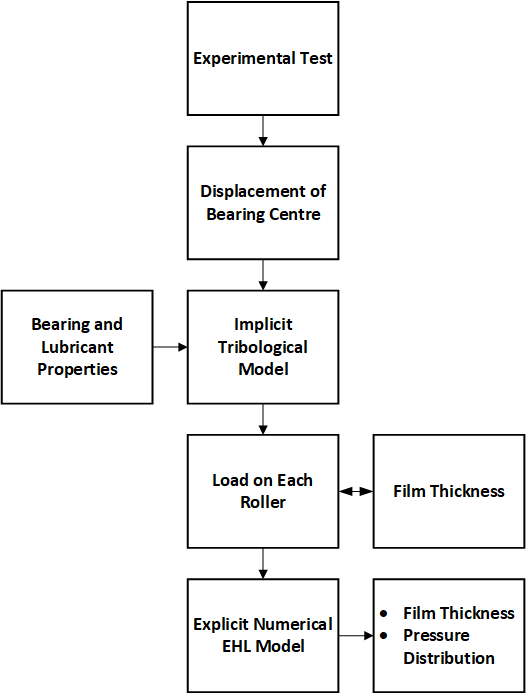
\includegraphics[width=100 mm]{ExpTribo Figure 1 - Methodology Overview.png}
	\caption{Experimental tribodynamics methodology overview.}
	\label{Experimental Tribodynamics Methodology Overview}
\end{figure}

\subsection{Operating Principles}

The rollers within a bearing carry an instantaneous share of the overall applied load \cite{Guo2020}. Deviation of the supported shaft from its nominal geometric centre results in a loaded region of the bearing. Due to the non-conformal nature of the contact between the bearing roller and race, these loads generate high pressures, leading to local surface deformation and increased lubricant viscosity. In conjunction with relative motion at the contact, this results in EHL film formation \cite{Gohar1988} \cite{Grubin1949}. In the unloaded region of the bearing, emerging clearances result in a shift to the hydrodynamic regime of lubrication, which can result in sliding and roller-cage collisions \cite{Mohammadpour2015c}. Hence, the contact may go through different regimes of lubrication throughout operation\cite{Denni2019}.

\begin{figure}
	\centering
	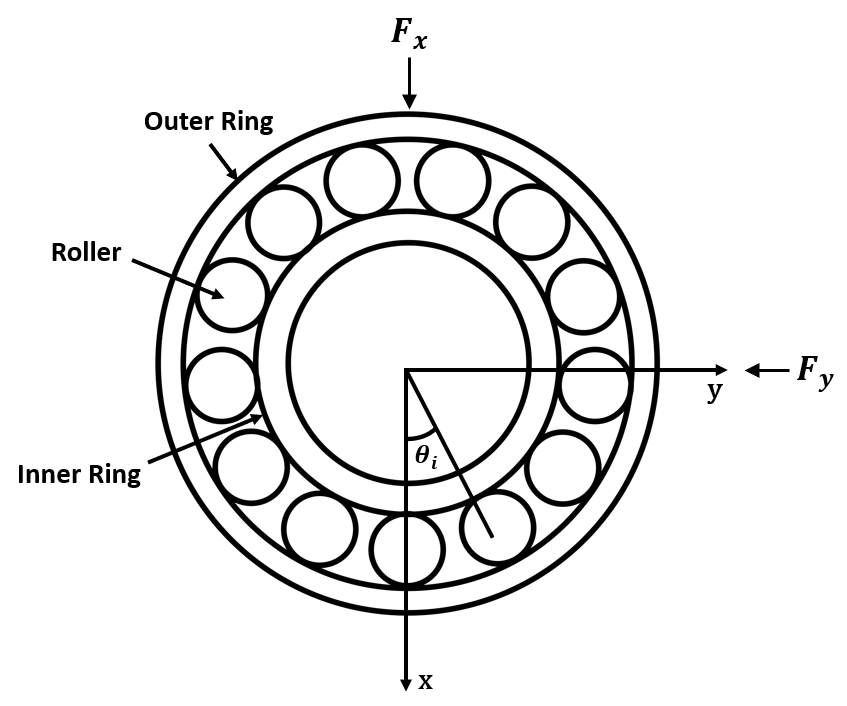
\includegraphics[width=100 mm]{ExpTribo Figure 2 - CRB in equilibrium position.png}
	\caption{Cylindrical roller bearing in equilibrium position.}
	\label{CRB in equilibrium position}
\end{figure}

Figure \ref{CRB in equilibrium position} shows a cylindrical roller bearing (CRB) in equilibrium position with zero preload or design clearance. In the absence of an applied radial load, $F_0$, the initial deformation, $\delta_o$, and radial clearance, $C_0$, between rollers and races are both zero. On application of external force, the resulting instantaneous radial load, $F_i$, will displace the inner bearing race from its equilibrium state ($\Delta x$ and $\Delta y$). By analysing an individual roller at its instantaneous angular position, $\theta_i$, the resultant displacement of the bearing centre can be used to determine the deflection at the roller-race contact, $\delta_i$. These contact deformations will result in contact forces, $W_i$, which maintain the roller and races in dynamic equilibrium. The above interpretation is valid considering rigid inner and outer races.

\begin{figure}
	\centering
	\includegraphics[width=150 mm]{ExpTribo Figure 3 – Mutual separation and convergence of inner and outer races 2.png}
	\caption{Mutual separation and convergence of inner and outer races.}
	\label{Mutual separation and convergence of inner and outer races}
\end{figure}

Figure \ref{Mutual separation and convergence of inner and outer races} presents the case whereby an instantaneous load is applied to the inner race. This causes deflection of the rollers in the loaded region and generates clearance around the rollers in the unloaded region. The deflections at the inner and outer race correspond to the normal component of the bearing centre's displacement at the instantaneous position of that roller. In the current study, this displacement was experimentally measured from the test rig and used quasi-statically as the boundary condition for the tribological model. It should be noted that this study considers in-plane, 2-DOF motion. This is a valid assumption under dominant vertical radial loading with secondary horizontal motion from the full system dynamics.

\subsection{Lubricated Contact Mechanics}

To calculate contact force based on deflection between the roller and race, the Hertzian load-deflection relationship is used. For low-speed, highly loaded analysis, the EHL film is typically neglected and the contact is considered dry. However, at high entrainment velocities, the literature study revealed that the EHL film also influences this contact force. The lubricant imposes additional deformation at the contact points which, changes the calculated force. Figure \ref{Dry vs lubricated roller-race contact} in Chapter \ref{Lubricated FMBD} demonstrates this graphically. 

In this study, the central film thickness at the roller-race conjunction is calculated using an extrapolated central film thickness formula. The impact of the film on deflection, and consequently contact force, is evaluated using an iterative approach due to the interdependence between contact load and film thickness. In this part of the workflow, the stiffness and damping of the EHL film is neglected due to its rigid-like stiffness, which is several orders of magnitude higher than the Hertzian contact \cite{Walford1983} \cite{Dareing1975} \cite{Mehdigoli1990}.

For detailed tribological investigations, the numerical solution of the fluid film is essential. This provides the pressure, film thickness and shear distributions at the contact. This allows for further evaluation of the durability and frictional efficiency of the system. In the current study, the load on the roller and contact kinematics obtained from the implicit bearing model is used explicitly in a 1D elastohydrodynamic model to obtain film thickness and pressure distribution for specific loading periods through the speed sweep, as is shown in Figure \ref{EHL film thickness and pressure distribution at contact}. Since misalignment along the length of the rollers is not considered due to the high stiffness of the shaft and bracket, the 1D EHL analysis is sufficient \cite{Gupta1979}. This explicit approach significantly improves the computational efficiency of the model by negating the requirement for an implicit numerical EHL calculation at each sampling point.

\begin{figure}
	\centering
	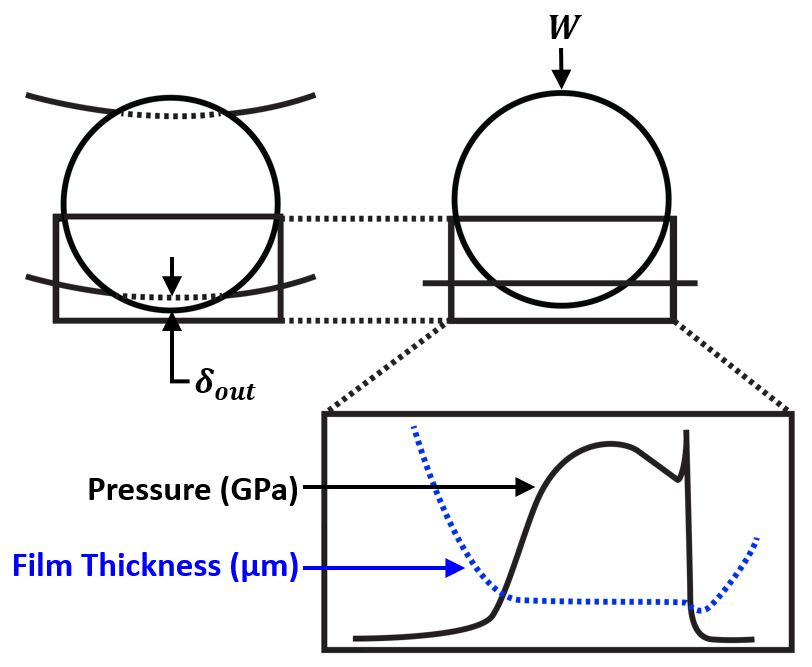
\includegraphics[width=100 mm]{ExpTribo Figure 4 - EHL film thickness and pressure distribution at contact.png}
	\caption{EHL film thickness and pressure distribution at contact.}
	\label{EHL film thickness and pressure distribution at contact}
\end{figure}

\subsection{Experimental Test Rig}

The displacement of the bearing centre governs the conditions at the contact and was found experimentally using a high-speed bearing test rig. A 5~kW AC synchronous motor, capable of speeds up to 32~000~rpm was coupled to a steel shaft that is supported by two bearing brackets. Radial force was transferred to the inner bearing race via the shaft using a hinge/arm mechanism and a point load application device on the shaft. Displacement data were obtained from an instrumented bearing bracket. Figure \ref{Experimental rig schematic} shows a schematic of the rig.

\begin{figure}
	\centering
	\includegraphics[width=120 mm]{ExpTribo Figure 5 – Experimental rig schematic.png}
	\caption{Experimental rig schematic.}
	\label{Experimental rig schematic}
\end{figure}

The motor control unit was connected to a voltage input, transmitted via an NI cDAQ-9178 USB chassis for optimum resolution of the input voltage. A MATLAB script controlled the voltage ramp over a specified time-period and thus the spindle acceleration. In this study, a transient speed sweep was performed from 0~–~15~000~rpm over a 4~s period, with 750~N of static radial load applied to the shaft. The bearing under test was a single row cylindrical roller bearing, NU~205~ECP, located in an aluminium test bracket that has an extruded bore for instrumentation.

\subsection{Instrumentation}
The outer surface of the bearing bore was instrumented with two Type~4383 single-axis piezo-electric charge accelerometers, with a frequency range of 0.1~–~8.5~kHz and sensitivity of 3.16~pC/ms2.  These measured acceleration of the bracket’s bore, corresponding to the outer race of the bearing (Figure \ref{Accelerometer locations on test bracket}). Two single beam laser vibrometers measured the displacement of the shaft at the edge of the bearing which corresponds to the displacement of the inner race of the bearing (Figure \ref{Laser vibrometer locations on shaft}). A dual-beam vibrometer was used to measure the rotational speed of the shaft. All laser vibrometers had a frequency range of 0~–~10~kHz and maximum speed of 20~000~rpm.

\begin{figure}
	\centering
	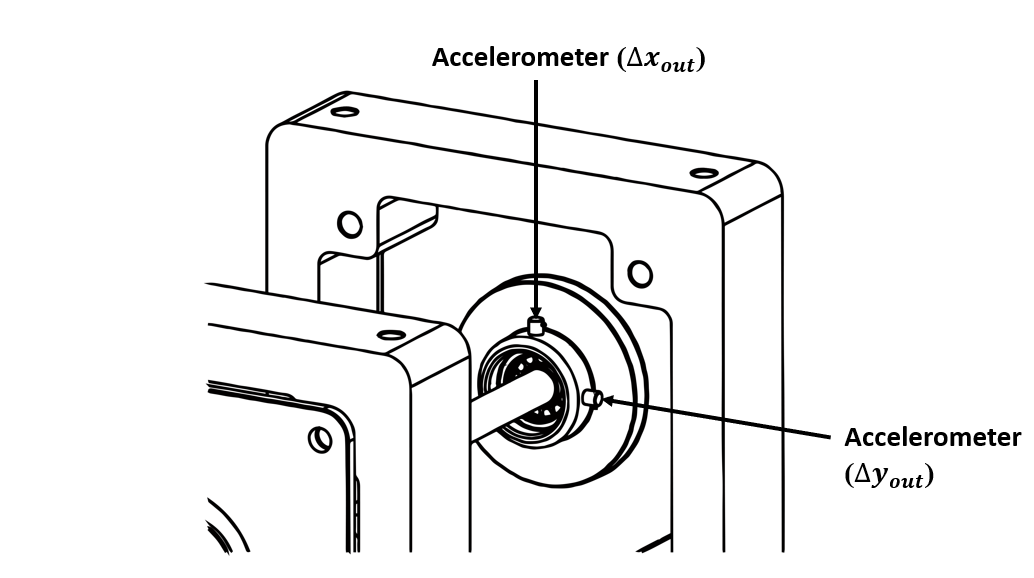
\includegraphics[width=150 mm]{ExpTribo Figure 6(a) - Accelerometer Locations on Test Bracket.png}
	\caption{Accelerometer locations on test bracket.}
	\label{Accelerometer locations on test bracket}
\end{figure}

\begin{figure}
	\centering
	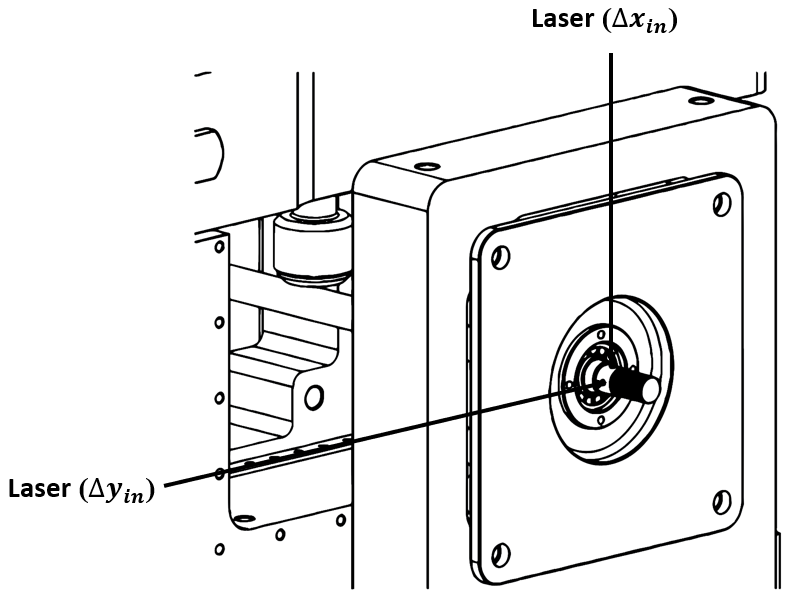
\includegraphics[width=120 mm]{ExpTribo Figure 6(b) Laser Vibrometer Locations on Shaft 2.png}
	\caption{Laser vibrometer locations on shaft.}
	\label{Laser vibrometer locations on shaft}
\end{figure}

A program in MATLAB controlled the speed of the shaft through a ramped voltage input. Data was simultaneously acquired from the accelerometers and laser vibrometers through synchronised input channels at a sampling rate of 100~kHz. Simultaneous control and data acquisition ensure accurate results between different instrumentation locations.

\subsection{Signal Processing}
The bearing race displacements were obtained from the instrumented bearing using time-domain data from the accelerometers and laser vibrometers. The laser vibrometer directly provided displacement data, whereas the accelerometer data required post-processing of acceleration data. To ascertain the displacement of the bearing bore and thus outer bearing race, the accelerometer results were integrated twice:

\begin{equation}\label{accelvelointeg}
	v_{out}\left(t\right)=v_{0,out}+\ \int_{0}^{t}{a_{out}\ dt}
\end{equation}

\begin{equation}\label{acceldispinteg}
	x_{out}\left(t\right)=x_{0,out}+\int_{0}^{t}{v_{out}\ dt}
\end{equation}

As this double integration amplifies non-linearities in the original signal, it requires pre-processing \cite{Takeda2014}. Low frequency drift is removed from the unfiltered time-domain data by applying a linear fit to the data and then removing the trend from it.  

To extract the frequency content of the speed ramp, waterfall plots were generated using the accelerometer and laser vibrometer data. Short-time fast-Fourier transform (STFFT) was used, with data windows of six shaft rotations at each 100~rpm increment. The resulting signal was then filtered using a Butterworth bandpass filter for a frequency range of 70~-~10~000~$Hz$ to remove the high amplitude low frequency noise that was inherent to the equipment setup. The filter used 3~$dB$ of passband ripple and 7~$dB$ attenuation in the stopbands, which were set at 35~-~12~500~$Hz$.  
The relative displacement of the bearing centre could then be obtained from the relative displacement between the shaft (measured using the single beam laser vibrometer) and bearing bore:

\begin{equation}\label{relativdispaccelx}
	\Delta x = \Delta x_{in} - \Delta x_{out}
\end{equation}

\begin{equation}\label{relativdispaccely}
	\Delta y = \Delta y_{in} - \Delta y_{out}
\end{equation}

where $\Delta x_{in}$ and $\Delta x_{out}$ correspond to the displacements of the shaft and bearing bore respectively. 

\subsection{Contact Mechanics at the Roller Race Conjunction} \label{Contact mechanics experimental tribodynamics}

The contact between roller and race is modelled as an elastic deformation between an equivalent finite length elastic cylinder and rigid plate. This assumption is realistic under the conditions of an EHL line contact. The contact force on an individual roller at each instantaneous position, $W_i$, is obtained from the Hertzian load-deflection relationship:

\begin{equation}\label{Hertz load deflection}
	W_i=k \delta_i^n
\end{equation}

where $k$ is the Hertzian contact stiffness non-linearity between a rolling element and the inner or outer raceway groove. For the case of rolling element bearings, the exponent of localised deflection, $n$, is equal to $10/9$ \cite{Harris1984}. The contact deflection of a roller relative to the race, $\delta_i$, is due to the normal dynamic motion (i.e. the local mutual convergence) of the inner and outer bearing races, contribution of lubricant film thickness and any additional clearance or interference fit \cite{Mohammadpour2015c}. This is expressed as:

\begin{equation}\label{Contact deflection experimental}
	\delta_i=2\left(h_{c,i}-C\right)+x\cos{\left(\theta_i\right)}+y\sin(\theta_i)
\end{equation}

where $C$ is the local radial clearance, and $x$ and $y$ are the displacement components of the inner bearing race from its geometric centre. This normal approach between both races is the sum of the total deformation of the rollers and both races \cite{Hamrock1981}, hence:

\begin{equation}\label{Total deflection experimental}
\delta_i=\ \delta_{i,in}+\delta_{i,out}
\end{equation}

The equilibrium of forces in a system of stiffnesses in series is therefore:

\begin{equation}\label{Equilibrium of force experimental}
W_i=W_{i,out}=W_{i,in}
\end{equation}

To find the individual deflection of each contact due to differences in contact stiffness, the following relationship is used:

\begin{equation}\label{Individual deflection of contacts experimental}
{\delta_{i,in}}k_i={\delta_{i,out}}k_{out}
\end{equation}

The deflection value at each contact based on the total deflection and relationship between contact stiffness is then found from Equations \ref{Total deflection experimental} and \ref{Individual deflection of contacts experimental} to give:

\begin{equation}\label{Deflection at each contact}
	\delta_{i, \text { out }}=\frac{\delta_i}{\left(\frac{k_{\text {out }}}{k_{\text {in }}}\right)^{\frac{1}{n}}+1}
\end{equation}

The normal stiffness of the inner and outer races differs due to their geometry. To calculate the stiffness at each contact, the following equation is used: 

\begin{equation}\label{Contact stiffness experimental}
	\delta=\frac{F}{\pi E_r L}\left[\ln \left(\frac{4 \pi E_r R_{z x} L}{F}\right)-1\right]
\end{equation}

The deflection for a range of loads is calculated based on the geometry and material properties at the inner and outer race contacts. This non-linear relationship is numerically obtained and then curve fitted and represented by a power function in the form $F=a\delta^b$, with $b=10/9$ and a representing the contact stiffness. Individual contact stiffness and deflection at the inner and outer race contacts is then found. The overall contact stiffness, $K_{i,total}$, is given by:

\begin{equation}\label{Overall contact stiffness}
	K_{i, \text { total }}=\frac{1}{\left(\frac{1}{K_{i, \text { in }}}\right)+\left(\frac{1}{K_{i, \text { out }}}\right)}
\end{equation}

where $K_{i,in}$ and $K_{i,out}$ are the stiffnesses of the inner and outer race contacts respectively.

\subsection{Implicit Tribological Model}

A stepwise solution was performed on an individual roller at each orbital position. The roller bearing and bracket tolerances are such that the internal clearance is $0~\mu m$ between roller and race. In an unloaded state, there is no deflection of elements or raceway. Displacement in positive $x-y$ corresponds to the same total magnitude of deflection of roller and race contacts. For each time step, the bearing is first assumed to be in equilibrium position and film thickness is assumed to be 0~$\mu m$. The deflection of the bearing is calculated under these conditions and is therefore a function of the relative displacement between inner and outer bearing races. With deflection at the time step calculated, the resultant lubricant regime and subsequent analytical solutions can be performed based on the following three conditions:

\begin{enumerate}
	\item $\delta=0$ indicates a film of 0 $\mu m$ and no load.
	\item $\delta<0$ indicates complete separation of the roller and race. In this instance, the lubricant is assumed to fill the separation gap, with the film thickness value equalling the magnitude of the separation:
	
	\begin{equation}\label{hydrodynamic film thickness}
		h_i=\left|\delta_i\right|
	\end{equation}

	Under this condition, the lubrication is in the hydrodynamic regime. The hydrodynamic lubricant reaction load was derived by Rahnejat \cite{Rahnejat1984}, and is given by:
	
	\begin{equation}\label{hydrodynamic reaction load}
		W_i=\frac{2 b u_i \eta_0 R_{z x}}{h_i}
	\end{equation}

	where $b$ is the half length of the contact, $u_i$ is the speed of lubricant entrainment into the contact, $\eta_0$ is the lubricant viscosity, $R_{zx}$ is the reduced radius of the roller and race and $h$ is lubricant film thickness. 
	
	\item $\delta>0$ indicates deflection at the roller-race contact. This means that contact pressure is sufficiently high for the lubrication regime to be elastohydrodynamic. For the elastohydrodynamic regime, an iterative process is performed to solve the film thickness. This is due to the contribution of EHL film towards deformation and consequently the load in the contact.
	
	The cylindrical roller and race contacts are modelled by an equivalent rigid roller against a semi-infinite elastic half space of equivalent elastic modulus, $E_r$. The extrapolated central film thickness for a line contact is therefore obtained \cite{Dowson1979} from:  
	
	\begin{equation}\label{dimensionless central film thickness}
	h_c=R_{zx}\left[{3.06G}^{\ast0.56}{U^{\ast0.69}W}^{\ast-0.1}\right]
    \end{equation}

	where the following dimensionless parameters are used:
		
	\begin{equation}\label{Gstar}
		G^*=\alpha E_r 
	\end{equation}
	
	\begin{equation}\label{Ustar}
		U^*=\frac{u \eta_0}{R_{z x} E_r}
	\end{equation}
	
	\begin{equation}\label{Wstar}
		W^*=\frac{w}{L E_r R_{z x}}
	\end{equation}

	where $R$ is the reduced radius of the contact, $L$ is the length of the roller and $u$ is the speed of entraining motion into the contact and $W$ is the contact load. Assuming pure rolling, the speed of entraining motion is given by:
	
	\begin{equation}\label{entraining motion speed}
		u_i=\frac{1}{2}\left(\omega_{c, i}-\omega_{r i, i}\right) r_{i n}
	\end{equation}

	An iterative process is used to calculate load on the roller based on total deflection including lubricant film (Equation \ref{Contact deflection experimental}). At each time step where an EHL film is present, the following convergence criteria must be met before the next time step is calculated:
	
	\begin{equation}\label{film convergence}
		\frac{h_i^n-h_i^{n-1}}{h_i^{n-1}} \leq 0.01
	\end{equation}

\end{enumerate}

\subsection{Surface Topography Measurements} \label{Surface Topography}

To assess the likelihood of asperity interaction, the roughness height of asperities, ${\sigma}$, must be measured for the roller and race. Surface topography measurements were performed using an Alicona InfiniteFocus Variation Microscope with a $\times 10$ objective. This had a vertical resolution of 30 $nm$ and sampling point separation of 176.9 $nm$ in the $y-z$ plane of the roller and 1 $nm$ in $x$. An area of 530 by 588 $\mu m$ was captured. Data was processed using Vision65 Map Premium software, where the profile radius of the roller and race was removed. The measured parameters for a roller and race are presented in Table \ref{Surface Topography Data}. The resulting composite surface roughness of a roller-race contact is 0.207 $\mu m$.


\begin{table*}
	\caption{Surface topography data}
	\label{Surface Topography Data}
	\centering
	\renewcommand{\arraystretch}{1.5}%
	\begin{tabular}{|p{5.5cm}<{\centering}|p{3.5cm}<{\centering}|p{3.5cm}<{\centering}|}
		\hline 
		\multirow{2}{*}{\textbf{Parameter}} & \multicolumn{2}{|c|}{\textbf{Value}} \\ 
		\cline { 2 - 3 } 
		& \textbf{Roller} & \textbf{Inner race} \\
		\hline 
		Root-mean-square height & 0.197 $\mu m$ & 0.065 $\mu m$ \\
		\hline 
		Density of peaks& 0.00116 $\mu \mathrm{m}^-2$ & 0.00153 $\mu \mathrm{m}^{-2}$  \\
		\hline 
		Arithmetic mean peak curvature & 0.180 $\mu \mathrm{m}^{-1}$ & 0.038 $\mu \mathrm{m}^{-1}$ \\
		\hline 
	\end{tabular}
\end{table*}


\section{Numerical EHL Model}\label{1D EHL Model}

Whilst the analytical solution used in the implicit tribological model provides central film thickness, the film thickness and pressure distributions can only be obtained explicitly through the full solution of Reynolds equation in conjunction with rheological and elastic field models. In a line contact, where contact dimensions in the side-leakage direction, $y_c$, are much larger than the direction of entraining motion, $x_c$, pressure in $y_c$ direction is assumed constant due to the negligible gradient and the contact can be analysed in one dimension. This assumption is valid in the contact apart from small regions near the edge. A simplified 1D version of Reynolds equation can therefore be used \cite{Gupta1979}.

\subsection{Reynolds Equation}

Reynold’s equation \cite{Reynolds1886} is the governing equation of fluid film lubrication theory. For Newtonian fluids it can be derived from the full Navier-Stokes equations making the following assumptions, primarily the neglection of inertial forces and only retaining viscous forces on the lubricant \cite{Gohar1988}:
\begin{enumerate} % REQUIRES DIRECTIONS ADDING
	\item Body forces are negligible (mass of film is negligible)
	\item Pressure is constant through the lubricant film (z-direction) due to the thin film (dimensions of the region of pressure are typically 100 times the central film thickness).
	\item No slip at the boundaries
	\item Lubricant flow is laminar (low Reynolds number)
	\item Inertia and surface tension forces are negligible compared with viscous forces (working fluid has low mass and low acceleration)
	\item Shear stress and velocity gradients are only significant across the lubricant film
	\item The lubricant behaves as a Newtonian fluid
	\item Lubricant viscosity is constant across the film
	\item The lubricant boundary surfaces are parallel or at a small angle with respect to each other
\end{enumerate}

Reynolds equation is a second order, non-linear partial differential equation. It is made up of the pressure induced terms (Poiseuille flow) and the boundary velocity-induced term (Couette flow). 

The simplified 1D version of Reynolds equation is given by:

\begin{equation}\label{eq3.1}
	\frac{\partial}{\partial x}\left[\frac{\rho h^{3}}{6 \eta}\left(\frac{\partial p}{\partial x}\right)-\rho h u\right]=2 \frac{\partial(\rho h)}{\partial t}
\end{equation}

To solve Reynolds equation numerically, it must first be discretized and then solved using the finite-difference method. The following procedure explains this discretization.

Due to the steady state nature of the investigations, with the absence of shock loading, the transient squeeze term can be removed:
\begin{equation}\label{eq3.2}
	\frac{\partial}{\partial x}\left[\frac{\rho h^{3}}{6 \eta}\left(\frac{\partial p}{\partial x}\right)-\rho h u\right]=0
\end{equation}

Due to the many orders of magnitude differences between lubricant film thickness (µm) and pressures (GPa), the numerical solution often becomes unstable. Dimensionless parameters are therefore defined to remove this instability. These are as follows:

\begin{equation}\label{eq3.3}
	\begin{aligned}
		U &=\frac{u}{u_{a v}} & \partial x &=a \partial X \\
		\mathrm{X} &=\frac{x}{\mathrm{a}} & \partial \rho &=\rho_{0} \partial \bar{\rho} \\
		\bar{\rho} &=\frac{\rho}{\rho_{0}} & \partial \eta &=\eta_{0} \partial \bar{\eta} \\
		\bar{\eta} &=\frac{\eta}{\eta_{0}} & \partial h &=\frac{a^{2}}{R_{z x}} \partial H \\
		\mathrm{H} &=\frac{h R_{x}}{a^{2}} & \partial p &=p_{h} \partial P \\
		\mathrm{P} &=\frac{p}{p_{h}} & \\
		\mathrm{~W}^{*} &=\frac{w}{E_{r} R_{z x} L} &
	\end{aligned}
\end{equation}

Terms in the simplified Reynolds equation are replaced with dimensionless parameters. Similar terms are then grouped and rearranged to give the final form:

\begin{equation}\label{eq3.4}
	\frac{\partial}{\partial X}\left[\frac{\bar{\rho} H^{3}}{6 \bar{\eta}}\left(\frac{\partial P}{\partial X}\right)\right]=\Psi\left[\frac{\partial}{\partial X} \bar{\rho} H U\right]
\end{equation}

where

\begin{equation}\label{eq3.5}
	\Psi=\frac{12 u_{a v} R_{z x}^{2} \eta_{0}}{p_{h}}
\end{equation}

Grouping terms for simplicity
\begin{equation}\label{eq3.6}
	M=\frac{\bar{\rho} H^{3}}{6 \bar{\eta}}
\end{equation}

\begin{equation}\label{eq3.7}
	Q=\bar{\rho} H
\end{equation}

Making substitutions
\begin{equation}\label{eq3.8}
	\frac{\partial}{\partial X}\left[M\left(\frac{\partial P}{\partial X}\right)\right]=\Psi \frac{\partial}{\partial X}[Q U
\end{equation}

\begin{equation}\label{eq3.9}
	\left[M \frac{\partial^{2} P}{\partial X^{2}}+\left(\frac{\partial M}{\partial X}\right) \frac{\partial P}{\partial X}\right]=\Psi\left[U \frac{\partial Q}{\partial X}+Q \frac{\partial U}{\partial X}\right]
\end{equation}

The final term is removed, as velocity, $U$, is independent of $x$ when no stretching of the surfaces occurs. This is then differentiated to give:

\begin{equation}\label{eq3.10}
	\frac{\partial M}{\partial X}=\frac{\partial}{\partial X}\left[\frac{\bar{\rho} H^{3}}{6 \bar{\eta}}\right]=\frac{H^{2}}{2 \bar{\eta}}\left[\left(\frac{H}{3}\right) \frac{\partial P}{\partial X}+\bar{\rho} \frac{\partial H}{\partial X}-\left(\frac{\bar{\rho} H}{2 \bar{\eta}}\right) \frac{\partial \bar{\eta}}{\partial X}\right]
\end{equation}

and

\begin{equation}\label{eq3.11}
	\frac{\partial Q}{\partial X}=\frac{\partial}{\partial X}[\bar{\rho} H]=H \frac{\partial \bar{\rho}}{\partial X}+\bar{\rho} \frac{\partial H}{\partial X}
\end{equation}

Substituting into Equation \ref{eq3.9} gives the following:

\begin{equation}\label{eq1.12}
	\frac{\bar{\rho} H^{3}}{6 \bar{\eta}} \frac{\partial^{2} P}{\partial X^{2}}+\frac{H^{2}}{2 \bar{\eta}}\left[\frac{H}{3} \frac{\partial \bar{\rho}}{\partial X}+\bar{\rho} \frac{\partial H}{\partial X}-\frac{\bar{\rho} H}{2 \bar{\eta}} \frac{\partial \bar{\eta}}{\partial X}\right] \frac{\partial P}{\partial X}-\Psi U\left[H \frac{\partial \bar{\rho}}{\partial X}+\bar{\rho} \frac{\partial H}{\partial X}\right]=0
\end{equation}

\begin{equation}\label{eq3.13}
	\frac{\partial^{2} P}{\partial X^{2}}+\frac{3}{\bar{\rho} H}\left[\frac{H}{3} \frac{\partial \bar{\rho}}{\partial X}+\bar{\rho} \frac{\partial H}{\partial X}-\frac{\bar{\rho} H}{2 \bar{\eta}} \frac{\partial \bar{\eta}}{\partial X}\right] \frac{\partial P}{\partial X}-\frac{6 \bar{\eta}}{\bar{\rho} H^{3}} \Psi U\left[H \frac{\partial \bar{\rho}}{\partial X}+\bar{\rho} \frac{\partial H}{\partial X}\right]=0
\end{equation}

The final form of the equation is therefore:

\begin{equation}\label{eq3.14}
	\frac{\partial^{2} P}{\partial X^{2}}+\left[\frac{1}{\bar{\rho}} \frac{\partial \bar{\rho}}{\partial X}+\frac{3}{H} \frac{\partial H}{\partial X}-\frac{3}{2 \bar{\eta}} \frac{\partial \bar{\eta}}{\partial X}\right] \frac{\partial P}{\partial X}-\frac{6 \bar{\eta}}{H^{2}}\left[\frac{1}{\bar{\rho}} \frac{\partial \bar{\rho}}{\partial X}+\frac{1}{H} \frac{\partial H}{\partial X}\right] \Psi U=0
\end{equation}

\subsection{Finite Difference Formulation} \label{Finite Difference Formulation}

To solve Reynolds equation computationally, a finite difference formulation required. The central difference formula based on Taylor series expansion \cite{Hoffmann2000} is used. The second derivative of pressure using second order central discretization for the spatial domain is therefore:

\begin{equation}\label{eq3.15}
	\frac{\partial^2 P}{\partial X^2}=\frac{P_{i-1}-2 P_i+P_{i+1}}{\Delta X^2}
\end{equation}

and the first derivative is given by:

\begin{equation}\label{eq3.16}
	\frac{\partial P}{\partial X}=\frac{P_{i+1}-P_{i-1}}{2 \Delta X}
\end{equation}

Replacing terms in the final form of discretized Reynold equation:

\begin{equation}\label{eq3.17}
	\frac{P_{i-1}-2 P_i+P_{i+1}}{\Delta X^2}+\left[\frac{1}{\bar{\rho}} \frac{\partial \bar{\rho}}{\partial X}+\frac{3}{H} \frac{\partial H}{\partial X}-\frac{3}{2 \bar{\eta}} \frac{\partial \bar{\eta}}{\partial X}\right] \frac{P_{i+1}-P_{i-1}}{2 \Delta X}-\frac{6 \bar{\eta}}{H^2}\left[\frac{1}{\bar{\rho}} \frac{\partial \bar{\rho}}{\partial X}+\frac{1}{H} \frac{\partial H}{\partial X}\right] \Psi U=0
\end{equation}

\begin{equation}\label{eq3.18}
	\frac{P_{i-1}+P_{i+1}}{\Delta X^2}+\left[\frac{1}{\bar{\rho}} \frac{\partial \bar{\rho}}{\partial X}+\frac{3}{H} \frac{\partial H}{\partial X}-\frac{3}{2 \bar{\eta}} \frac{\partial \bar{\eta}}{\partial X}\right] \frac{P_{i+1}-P_{i-1}}{2 \Delta X}-\frac{6 \bar{\eta}}{H^2}\left[\frac{1}{\bar{\rho}} \frac{\partial \bar{\rho}}{\partial X}+\frac{1}{H} \frac{\partial H}{\partial X}\right] \Psi U=\frac{2 P_i}{\Delta X^2}
\end{equation}

Pressure at each node point can then be represented by:

\begin{equation}\label{eq3.19}
	P_i=\frac{\frac{P_{i-1}+P_{i+1}}{\Delta X^2}+\left[\frac{1}{\bar{\rho}} \frac{\partial \bar{\rho}}{\partial X}+\frac{3}{H} \frac{\partial H}{\partial X}-\frac{3}{2 \bar{\eta}} \frac{\partial \bar{\eta}}{\partial X}\right] \frac{P_{i+1}-P_{i-1}}{2 \Delta X}-\frac{6 \bar{\eta}}{H^2}\left[\frac{1}{\bar{\rho}} \frac{\partial \bar{\rho}}{\partial X}+\frac{1}{H} \frac{\partial H}{\partial X}\right] \Psi U}{2\left(\frac{1}{\Delta X^2}\right)}
\end{equation}

Simplified to 

\begin{equation}\label{eq3.20}
	P_i=\frac{P_{x x}+P_x-E}{2\left(\frac{1}{\Delta X^2}\right)}
\end{equation}

where

\begin{equation}\label{eq3.21}
	P_{x x}=\frac{P_{i-1}+P_{i+1}}{\Delta X^2}
\end{equation}

\begin{equation}\label{eq3.22}
	P_{x}=\frac{P_{i+1}-P_{i-1}}{2 \Delta X}\left[\frac{1}{\bar{\rho}} \frac{\partial \bar{\rho}}{\partial X}+\frac{3}{H} \frac{\partial H}{\partial X}-\frac{3}{2 \bar{\eta}} \frac{\partial \bar{\eta}}{\partial X}\right]
\end{equation}

\begin{equation}\label{eq3.23}
	E=\frac{6 \bar{\eta}}{H^2}\left[\frac{1}{\bar{\rho}} \frac{\partial \bar{\rho}}{\partial X}+\frac{1}{H} \frac{\partial H}{\partial X}\right] \Psi U
\end{equation}

\subsection{Effect of Pressure on Lubricant Viscosity}

EHL temperatures are typically in the region of 0.5~-~4~$GPa$. The resultant behaviour of the viscosity at these pressures is instrumental in forming the EHL film and must be accounted for. The Barus law \cite{Barus1893} determines viscosity increase with pressure assuming constant ambient temperature: 

\begin{equation}\label{eq3.24}
	\eta=\eta_0 \exp (\alpha p)
\end{equation}

where $\eta$ is the lubricant viscosity at gauge pressure, $p$, $\eta_0$ is the viscosity at $p$~=~0, and $\alpha$ is the pressure-viscosity coefficient $({m}^2 /{N})$ and is specific to the lubricant. This relationship does not account for the change in $\alpha$ with temperature and pressure \cite{Gohar2019}, becoming inaccurate above 0.5~GPa.

A more comprehensive relationship which simultaneously includes the effects of temperature and pressure was one proposed by Roelands \cite{Roelands1966} and developed by Houpert \cite{Houpert1984}.  Roelands law is therefore accurate at higher contact pressures:

\begin{equation}\label{eq3.25}
    \eta=\eta_0 \exp \left(\alpha^* p\right)
\end{equation}

The Roelands pressure-viscosity coefficient, $\alpha^\ast$, is a function of both $p$ and $\theta$, with $\theta_0$ being the reference or ambient temperature, for example at the inlet:

\begin{equation}\label{eq3.26}
	\alpha^* p=\left[\ln \left(\eta_0+9.67\right)\right]\left\{\left(\frac{\theta-138}{\theta_0-138}\right)^{-S_0}\left[\left(1+\frac{p}{p_0}\right)^{Z_0}-1\right]\right\}
\end{equation}

where

\begin{equation}\label{eq3.27}
	z_0=\frac{\alpha}{5.1 \times 10^{-9}\left[\ln \left(\eta_0\right)+9.67\right]}
\end{equation}

and

\begin{equation}\label{eq3.28}
	S_0=\frac{\beta\left(\theta_0-138\right)}{\ln \left(\eta_0\right)+9.67}
\end{equation}

The oil constants $Z_0$ and $S_0$ are independent of both pressure and temperature, and $Z_0$ can be typically taken as 0.68 for computational purposes.

\subsection{Effect of Pressure on Lubricant Density}

For accurate film EHL film shape calculations, the effect that pressure has on the lubricant density must be considered. The most common equation for this is the widely used Dowson and Higginson model \cite{Dowson1977}:

\begin{equation}\label{eq3.29}
	\rho=\rho_0\left(1+\frac{0.6 \times 10^{-9} p}{1+1.7 \times 10^{-9} p}\right)
\end{equation}

where $\rho_0$ is the lubricant atmospheric pressure. Further modifications can be made to account for the effects of temperature:

\begin{equation}\label{eq3.30}
	\rho=\rho_0\left(1+\frac{0.6 \times 10^{-9} p}{1+1.7 \times 10^{-9} p}\right)\left[1-0.65 \times 10^{-3}\left(\theta-\theta_0\right]\right.
\end{equation}


\subsection{Effect of Temperature on Lubricant Viscosity}

Most EHL work assumes constant temperature of the contact and that viscosity and density are dependent on pressure only. Standard experiments have been performed to assess effect of temperature on viscosity. Results have previously been curve fit by Crouch and Cameron \cite{Crouch1961}, with the most simple fit due to Reynolds:

\begin{equation}\label{eq3.31}
	\eta=\eta_s \exp (-\beta \Delta \theta)
\end{equation}

where $\eta_s$ is the viscosity of the lubricant at temperature $\theta_s$, $\eta$ is the viscosity at representative temperature, $\theta$, and $\Delta \theta$ represents the temperature difference between the two. $\beta$ is the thermoviscous constant and is lubricant specific. This relationship is only valid for small temperature rises of the lubricant. A more accurate and widely used equation is the expression from Vogel:

\begin{equation}\label{eq3.32}
	\eta=K \exp \left(\frac{b}{\theta+c}\right)
\end{equation}

with the three constants dependant on the lubricant, obtained from knowing three pairs of values for $\theta$ and $\eta$.

\subsection{1D EHL Solution Methodology}

The methodology for the 1D EHL solution used within this thesis is as follows.

Reynolds equation is used to calculate contact pressures. Assuming a thin film of Newtonian lubricant in a line contact, the following form is used and discretized as described in Section \ref{Finite Difference Formulation}:

\begin{equation}\label{eq3.33}
	\frac{\partial}{\partial X}\left[\frac{\bar{\rho} H^3}{6 \bar{\eta}}\left(\frac{\partial P}{\partial X}\right)\right]=\Psi\left[\frac{\partial}{\partial X} \bar{\rho} H U\right]
\end{equation}

where $X$ is the direction of entraining motion into the contact. Squeeze film motion is neglected for this analysis. The pressure-density relationship in the compressible model is modelled using Dowson-Higginson \cite{Dowson1977} (\ref{eq3.29}). Roelands equation \cite{Roelands1966} (\ref{eq3.25}) is used for the pressure-viscosity relationship.

Pressure distribution is obtained from the variations in film thickness at the contact, which is defined as below:

\begin{equation}\label{eq3.34}
	h=h_0+\frac{x^2}{2 R_{z x}}-\frac{2}{\pi E_r} \int_{x_{c, \text { in }}}^{x_{c, \text { out }}} p \ln \left(x-x^{\prime}\right)^2 d x^{\prime}
\end{equation}

where $h_0$ is the central film thickness, the second term represents an idealised film thickness parabola, with the final term representing the localised contact deflection. Central film thickness is first estimated using \cite{Dowson1979}:

\begin{equation}\label{eq3.35}
	h_0=R_{z x} 3.06 G^{* 0.56} U^{* 0.69} W^{*-0.1}
\end{equation}

\begin{equation}\label{eq3.36}
	G^*=\alpha E_r 
\end{equation}

\begin{equation}\label{eq3.37}
	U^*=\frac{u \eta_0}{R_{z x} E_r}
\end{equation}

\begin{equation}\label{eq3.38}
	W^*=\frac{w}{L E_r R_{z x}}
\end{equation}

Below, the method of solution for the numerical EHL model is provided:

\begin{enumerate} % Requires ammendments depending on where in the context of the thesis this is placed
	\item Input the load value obtained from the implicit tribological model for an instantaneous position as well as contact kinematics from experimental conditions.
	\item An initial estimation of lubricant film thickness, $h_0$ is made.
	\item Inlet and outlet distances are set to $-4.5a$ to $1.5a$ based on the contact half width calculation. This sets up the computational domain, and assumes fully flooded inlet conditions \cite{Hamrock1976}. 
	\item Pressure distribution and film thickness are obtained through simultaneous solutions of equations \ref{eq3.33} to \ref{eq3.35} using the dimensionless parameters defined in \ref{eq3.3}. The Newton-Raphson iterative scheme is used for speed and robustness of convergence \cite{Okumara1982}. Pressure convergence criterion is required for the iterative solution:
	\begin{equation}\label{eq3.39}
		\operatorname{Err}_{\text {pressure }}=\frac{\sum_{i=1}^n\left|p_{\text {new }}-p_{\text {old }}\right|}{\sum_{i=1}^n p_{\text {old }}} \leq \varepsilon_p
	\end{equation}

	where $\varepsilon_p$= 1 $\times 10^{-5}$.
	
	Under-relaxation is applied between successive iterations where the criterion is not met:
	\begin{equation}\label{Under relaxation}
		p_{\text {new }}=(1-\gamma) p_{\text {old }}+\gamma p_{\text {new }}
	\end{equation}

	where the under-relaxation factor is typically 0.01 $\le\gamma\le$ 0.8
	
	\item Hydrodynamic reaction load is calculated using the integration of pressure over the computational domain:
	
	\begin{equation}\label{Reaction load integration EHL}
		W_h=L \int p d x
	\end{equation}

	The total reaction from the hydrodynamic load should be equal to the total load share on the roller, $W_i$, obtained from the explicit tribological model. The following convergence criterion is applied:
	
	\begin{equation}
		\frac{\left|W_i-W_h\right|}{W_i} \leq \varepsilon_W
	\end{equation}

	where $\varepsilon_W$ = 0.001 
\end{enumerate}

\subsection{Numerical EHL Model Validation}
Conjunction level validation of the numerical method for solving the EHL film thickness and pressure distributions was performed using the work of Masjedi and Khonsari \cite{Masjedi2012}. These were validated against their smooth surface plots with no asperity pressure contribution. The dimensionless input parameters were $W^*$ = 1~$\times 10^{-4}$, $U^*$ = 1~$\times 10^{-11}$ and $G^*$~=~4500. The results shown in Figure \ref{EHL Pressure Validation Masjedi Khonsari} and Figure \ref{EHL Film Validation Masjedi Khonsari} show a good agreement between the model used in the study and the work of Masjedi and Khonsari for the dimensionless pressure, $P$, and dimensionless film thickness, $H$, respectively.

\begin{figure}
	\centering
	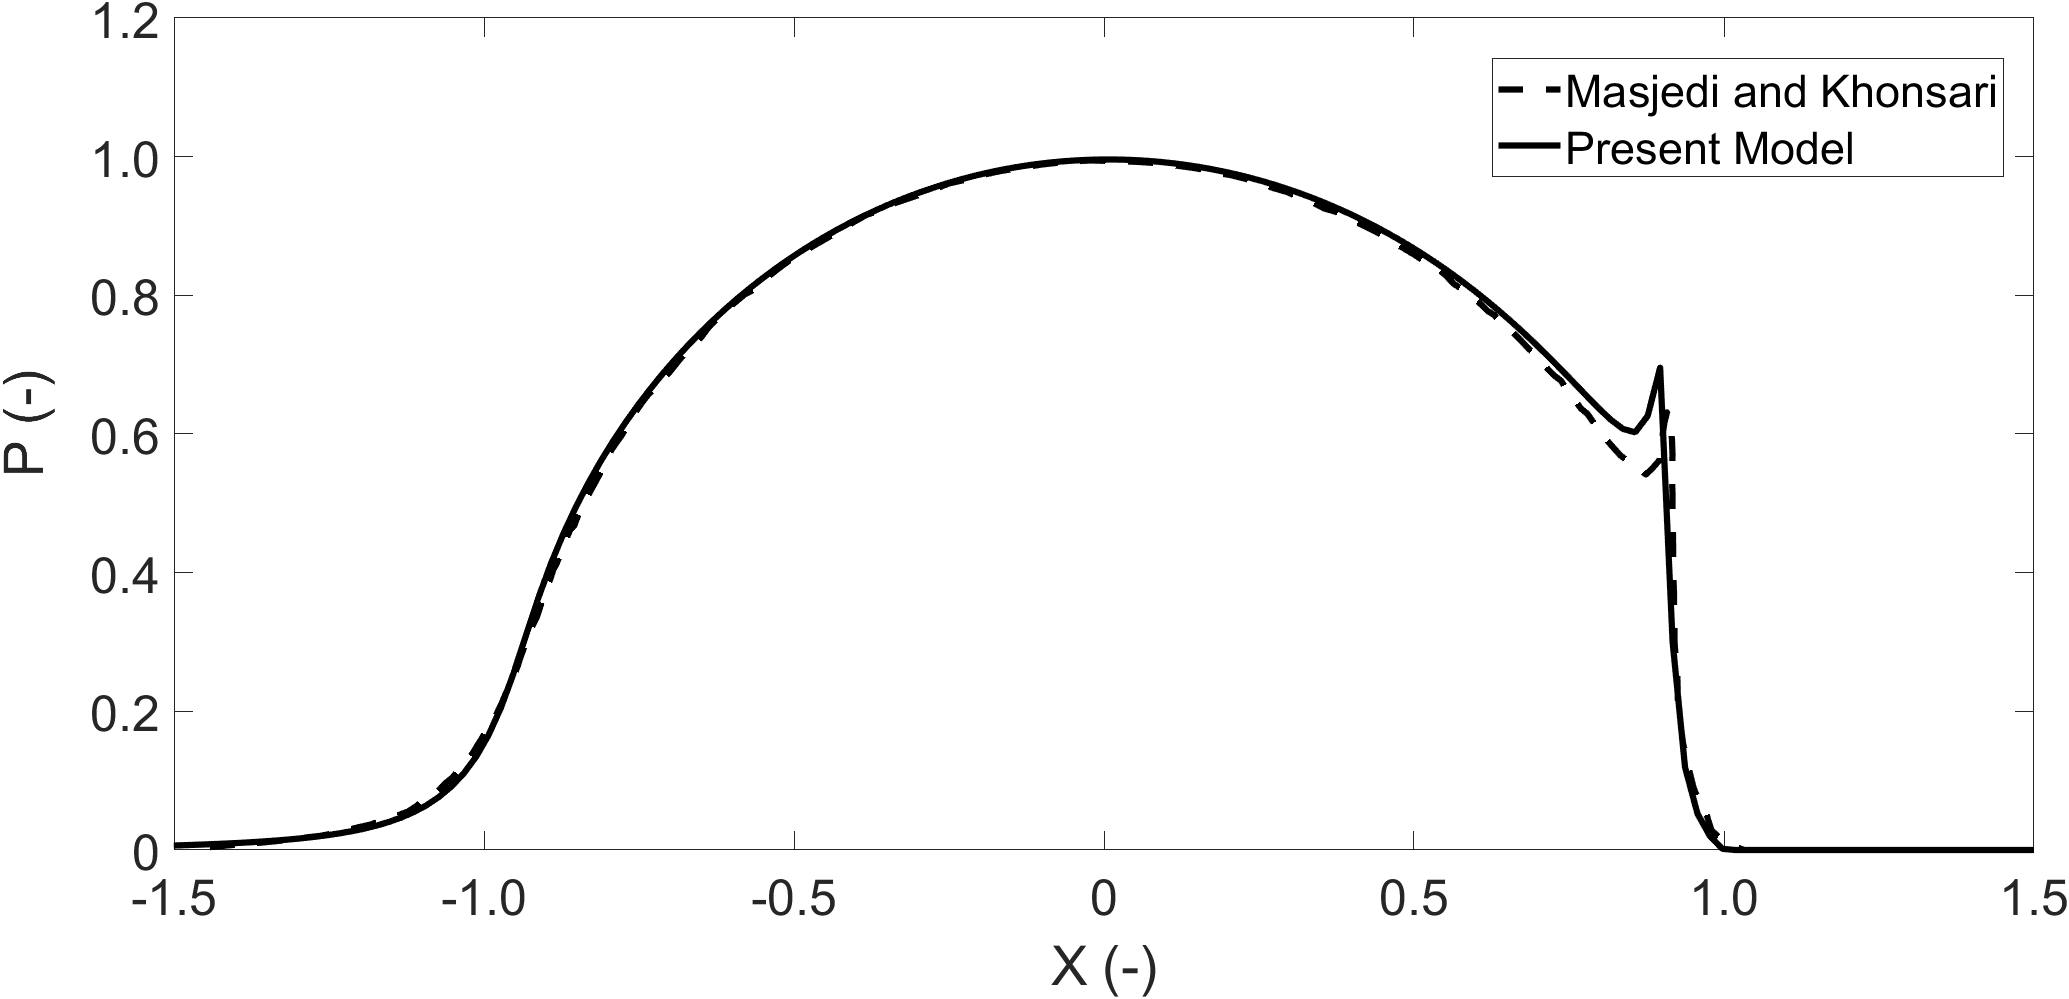
\includegraphics[width=120 mm]{ExpTribo Figure 9 - Validation of dimensionless pressure distribution, present model (solid), Masjedi and Khonsari (dashed).png}
	\caption{Validation of dimensionless pressure distribution, present model (solid), Masjedi and Khonsari (dashed).}
	\label{EHL Pressure Validation Masjedi Khonsari}
\end{figure}

\begin{figure}
	\centering
	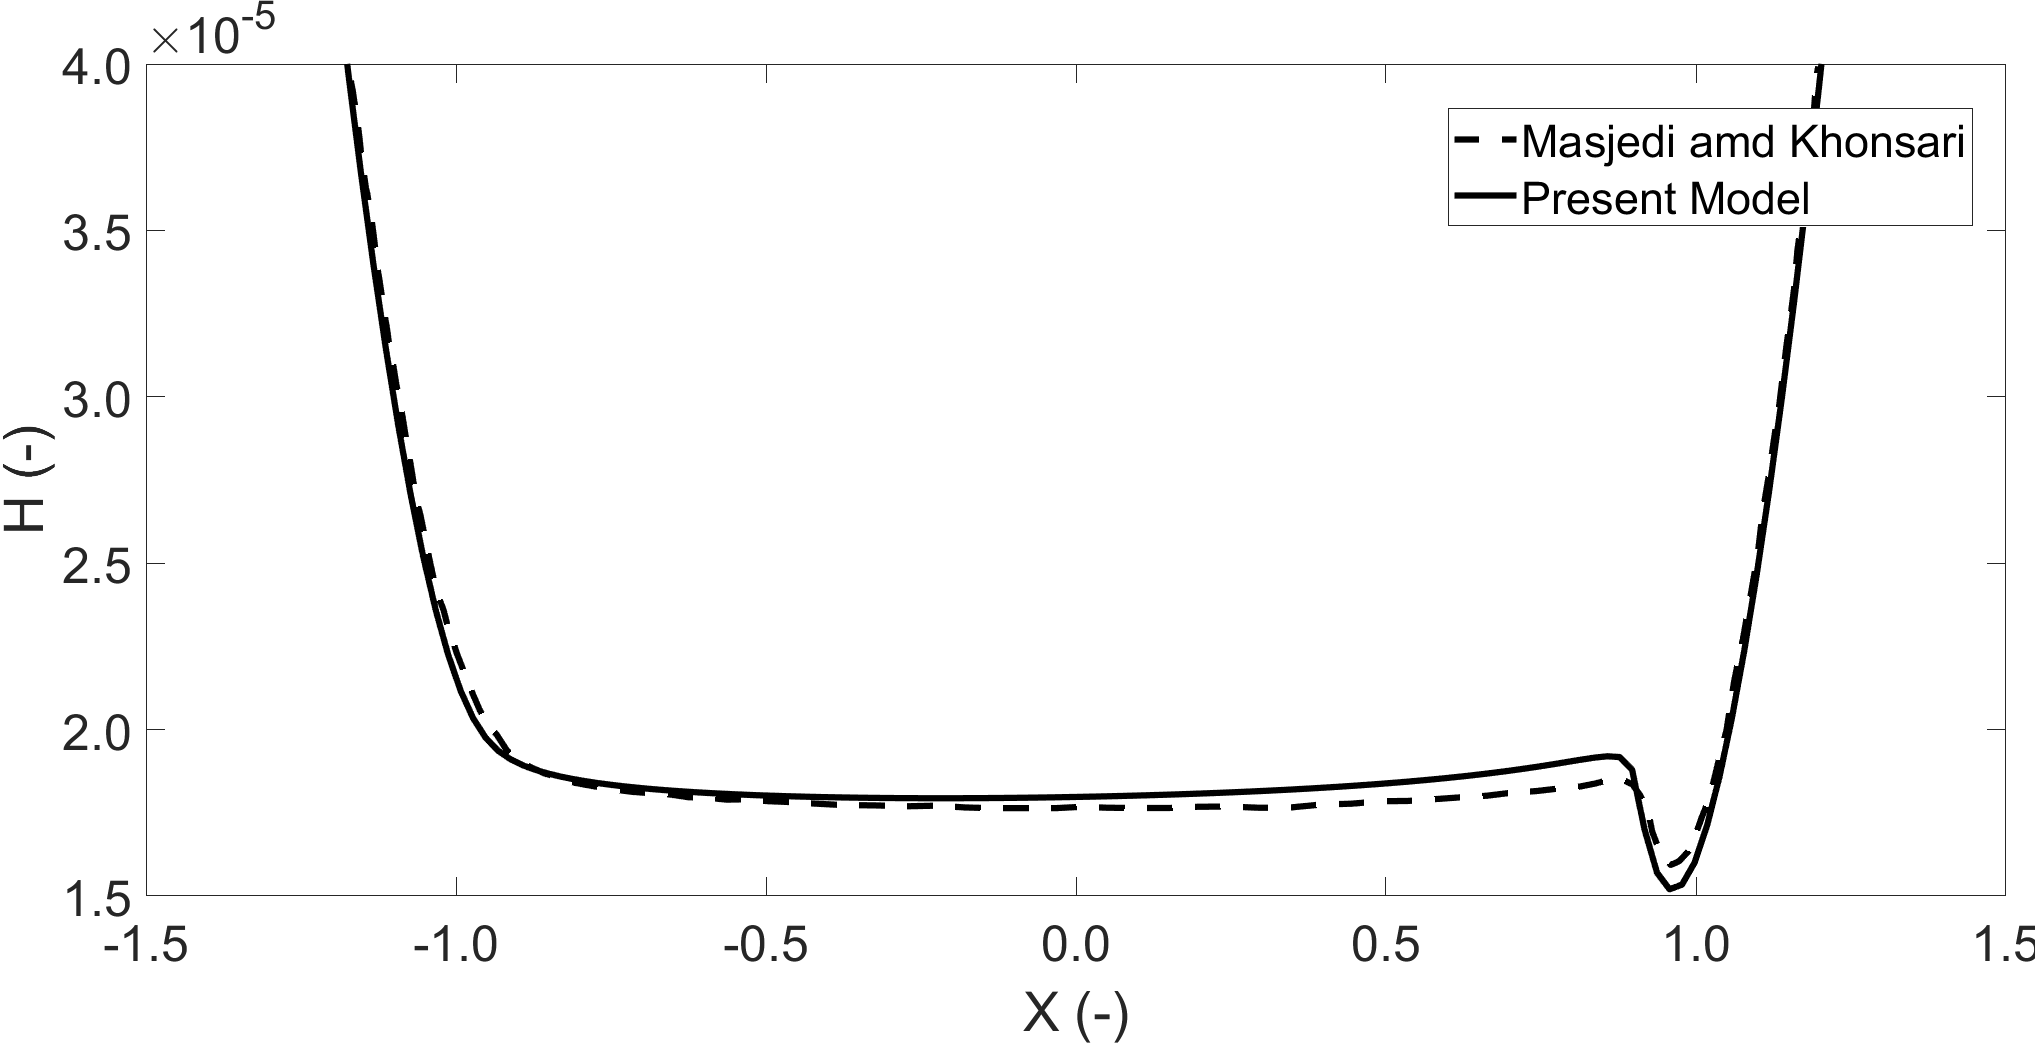
\includegraphics[width=120 mm]{ExpTribo Figure 10 - Validation of dimensionless film thickness distribution, present model (solid), Masjedi and Khonsari (dashed).png}
	\caption{Validation of dimensionless film thickness distribution, present model (solid), Masjedi and Khonsari (dashed).}
	\label{EHL Film Validation Masjedi Khonsari}
\end{figure}

\subsection{Experimental Result Verification}
The experimental results obtained from the presented rig were verified against analytically calculated frequency contents. This was to ensure the correct post processing of data for the input to tribological models. The bearing and lubricant data properties are given in Table \ref{Bearing Specification} and Table \ref{Lubricant and Material Properties} respectively.

\begin{table*}
	%\captionsetup{justification=centering}
	\caption{Bearing specification}
	\label{Bearing Specification}
	\centering
	\renewcommand{\arraystretch}{1.5}%
	\begin{tabular}{|c|c|}
		\hline
		\ \textbf{Parameter} & \textbf{Value} \\ [0.5ex]
		\hline
		Inner race bore & 25 $mm$ \\ [0.5ex]
		\hline
		Inner race diameter & 31.5 $mm$ \\ [0.5ex]
		\hline
		Outer race diameter & 46.5 $mm$ \\ [0.5ex]
		\hline
		Roller diameter & 7.5 $mm$ \\ [0.5ex]
		\hline
		Roller length & 9 $mm$ \\ [0.5ex]
		\hline
		Number of rollers & 12 \\ [0.5ex]
		\hline
		External load & 750 $N$ \\ [0.5ex]
		\hline
		Radial interference & 0 $\mu m$ \\ [0.5ex]
		\hline
	\end{tabular}
\end{table*}

\begin{table*}
	%\captionsetup{justification=centering}
	\caption{Lubricant and material properties}
	\label{Lubricant and Material Properties}
	\centering
	\renewcommand{\arraystretch}{1.5}%
	\begin{tabular}{|c|c|}
		\hline
		\ \textbf{Parameter} & \textbf{Value} \\ [0.5ex]
		\hline
		Pressure viscosity coefficient ($\alpha$) & 2.1 $\times 10^{-8}\mathrm{~Pa}^{-1}$ \\ [0.5ex]
		\hline
		Atmospheric lubricant dynamic viscosity & 0.08 Pa.s \\ [0.5ex]
		\hline
		Lubricant inlet density ($\rho_0$) & 833.8 $\mathrm{~kg}\cdot\mathrm{m}^{-3}$ \\ [0.5ex]
		\hline
		Eyring stress ($\tau_0$) & 2 $MPa$ \\ [0.5ex]
		\hline
		Shear strength of asperities ($\varsigma$) & 0.3 \\ [0.5ex]
		\hline
		Thermal conductivity of fluid & 1600 $\mathrm{~W}\cdot\mathrm{m}^{-1}\cdot\mathrm{K}^{-1}$ \\ [0.5ex]
		\hline
		Modulus of elasticity of contacting solids & 210 GPa \\ [0.5ex]
		\hline
		Poisson’s ratio of contacting solids & 0.3 \\ [0.5ex]
		\hline
        Density of contacting solids & 7850 $\mathrm{~kg}\cdot\mathrm{m}^{-3}$ \\ [0.5ex]
		\hline
		Thermal conductivity of contacting solids & 46 $\mathrm{~W}\cdot\mathrm{m}^{-1}\cdot\mathrm{K}^{-1}$ \\ [0.5ex]
		\hline
		Specific heat capacity of contacting solids & 470 $\mathrm{~J}\cdot\mathrm{kg}^{-1}\cdot\mathrm{K}^{-1}$ \\ [0.5ex]
		\hline
	\end{tabular}
\end{table*}

Primary frequencies in the system due to the interaction of the rolling elements, races and the shaft could be verified. These frequencies were calculated analytically, with $f_{bpi}$ and $f_{bpo}$ representing the ball pass frequencies of the inner and outer race respectively and $f_{shaft}$ being the rotational frequency of the shaft:

\begin{equation}\label{ball pass frequency inner}
	f_{b p i}=\frac{\omega_s}{2 \pi} \frac{N}{2}\left(1-\frac{D_r}{D_p}\right)
\end{equation}

\begin{equation}\label{ball pass frequency outer}
	f_{b p o}=\frac{\omega_s}{2 \pi} \frac{N}{2}\left(1+\frac{D_r}{D_p}\right)
\end{equation}

\begin{equation}\label{ball pass frequency shaft}
	f_{\text {shaft }}=\frac{\omega_s}{2 \pi}
\end{equation}

At 14~000~$rpm$, the theoretical inner and outer race frequencies are calculated to be 1669~$Hz$ and 1131~$Hz$ respectively, with the experimental results being 1611~$Hz$ and 1131~$Hz$. The first order shaft rotational frequency from the experiment was 232~$Hz$ compared to theoretical calculation of 233~$Hz$. The above frequencies can be seen clearly in Figure 7, which shows the bearing bore displacement spectra, and Figure 8 which represents the shaft displacement spectra. The verification frequencies are identical in both, confirming that the bearing motion is accurately measured by the experimental methodology. It is observed that at certain speeds, the ball pass frequency of the outer race has a larger contribution than the inner race. This is particularly highlighted at 12~000~-~14~000~$rpm$. These regional effects are contributed by modal behaviour of the bracket and the bed. The critical speed of the unloaded shaft, where lateral bending frequency of the shaft is equal to the rotation frequency \cite{Shigley'sMechanicalEngineeringDesign}, occurs at 12~660~$rpm$ and 211~$Hz$.

\begin{figure}
	\centering
	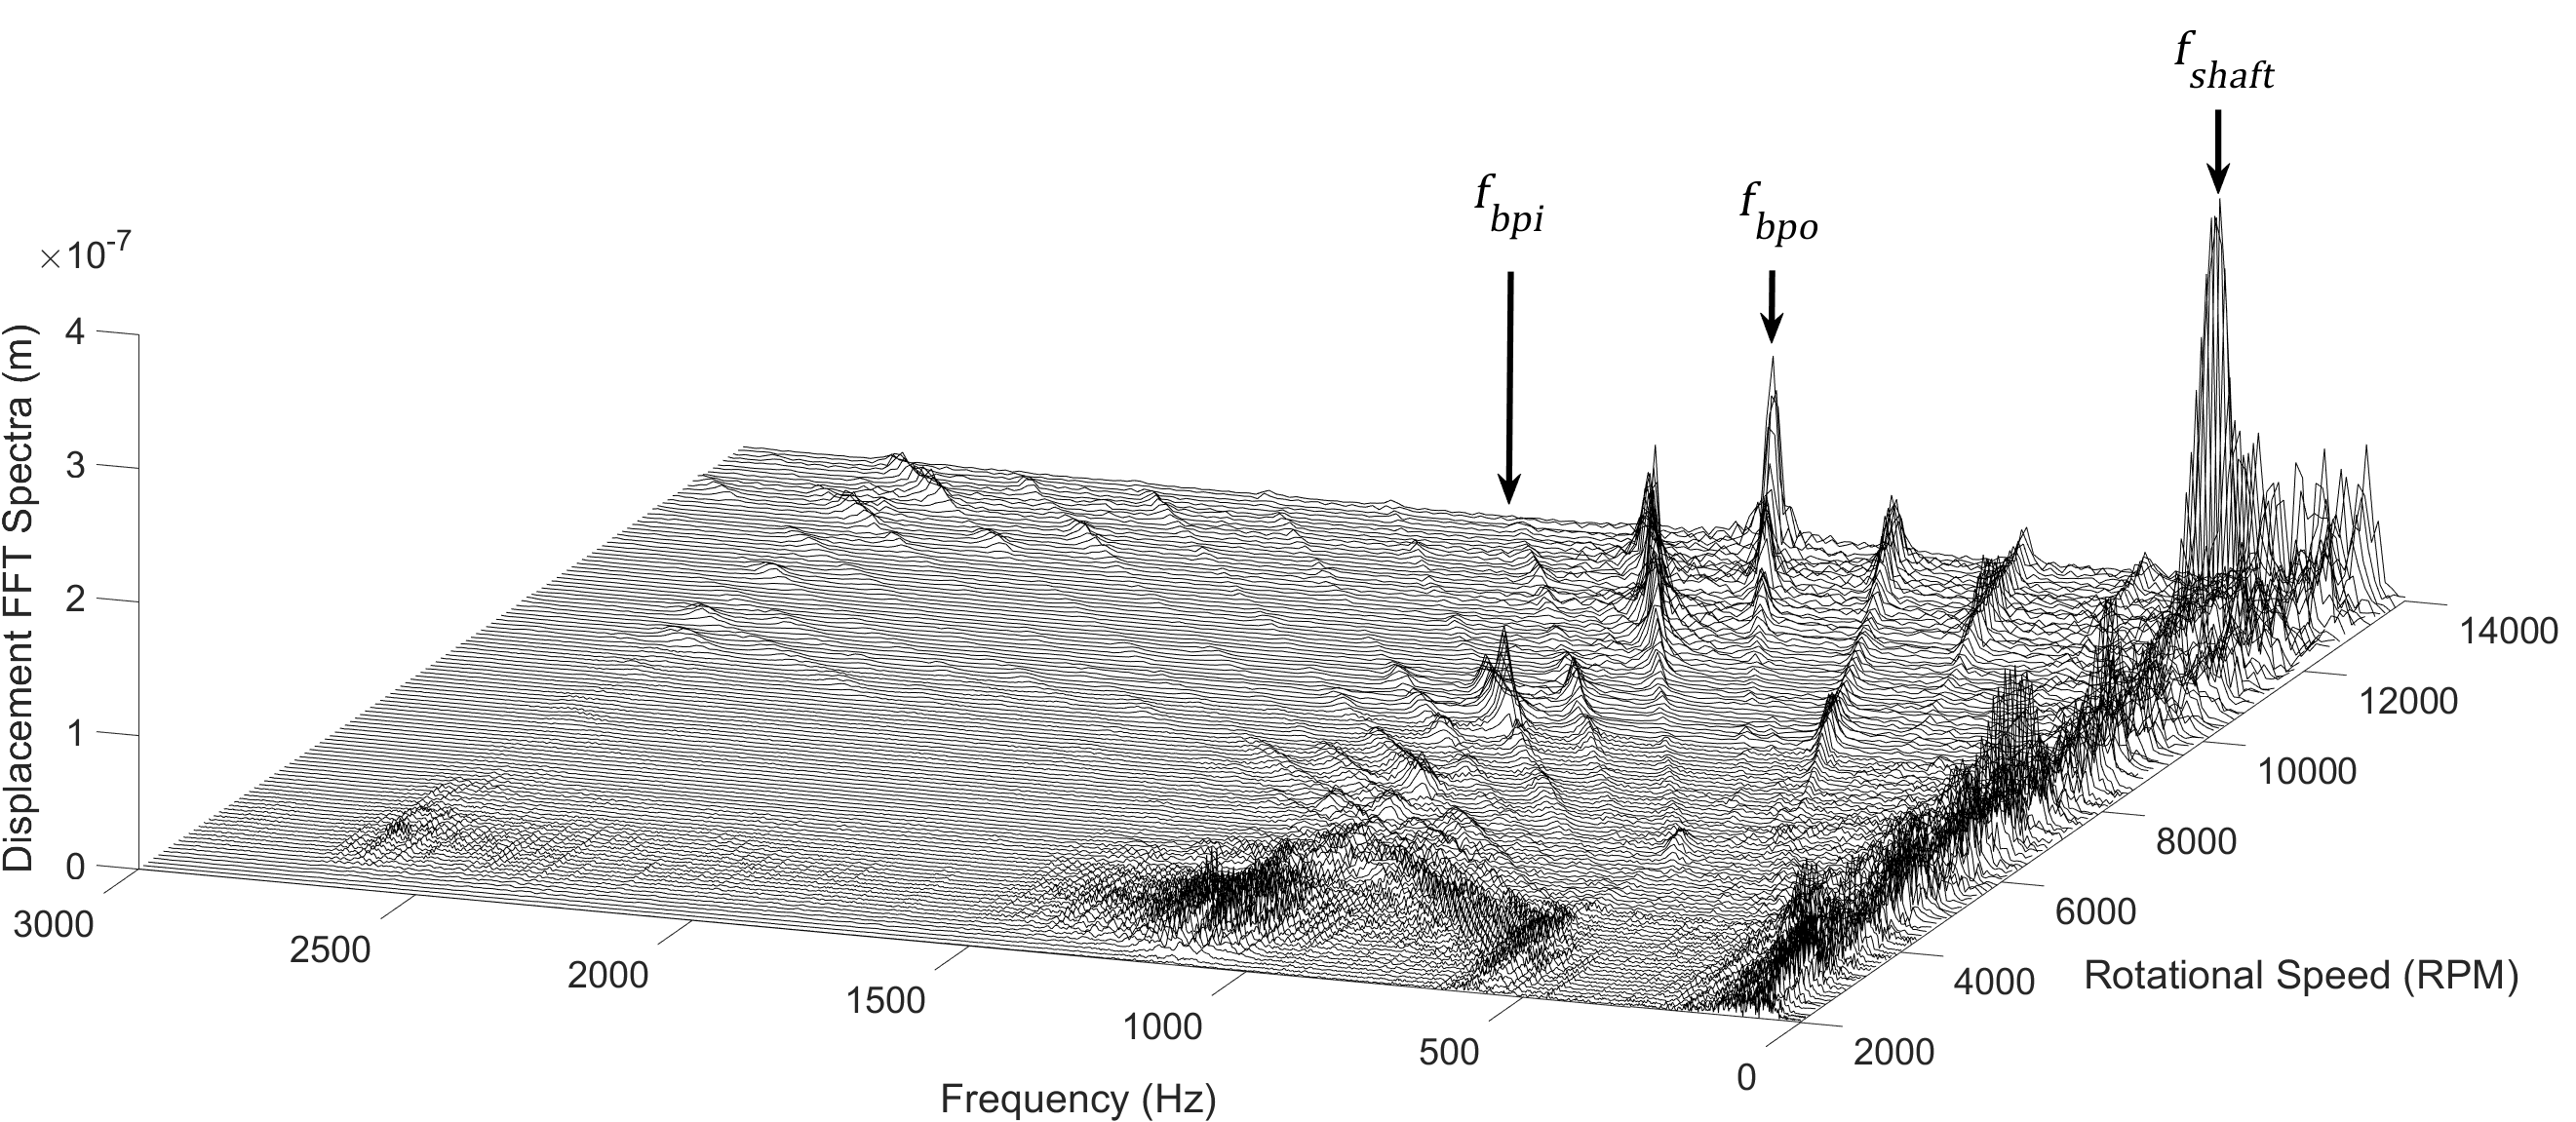
\includegraphics[width=150mm]{ExpTribo Figure 7 - Bearing Bore Displacement Frequency Spectra.png}
	\caption{Bearing bore displacement frequency spectra.}
	\label{Bearing bore displacement frequency spectra}
\end{figure}

\begin{figure}
	\centering
	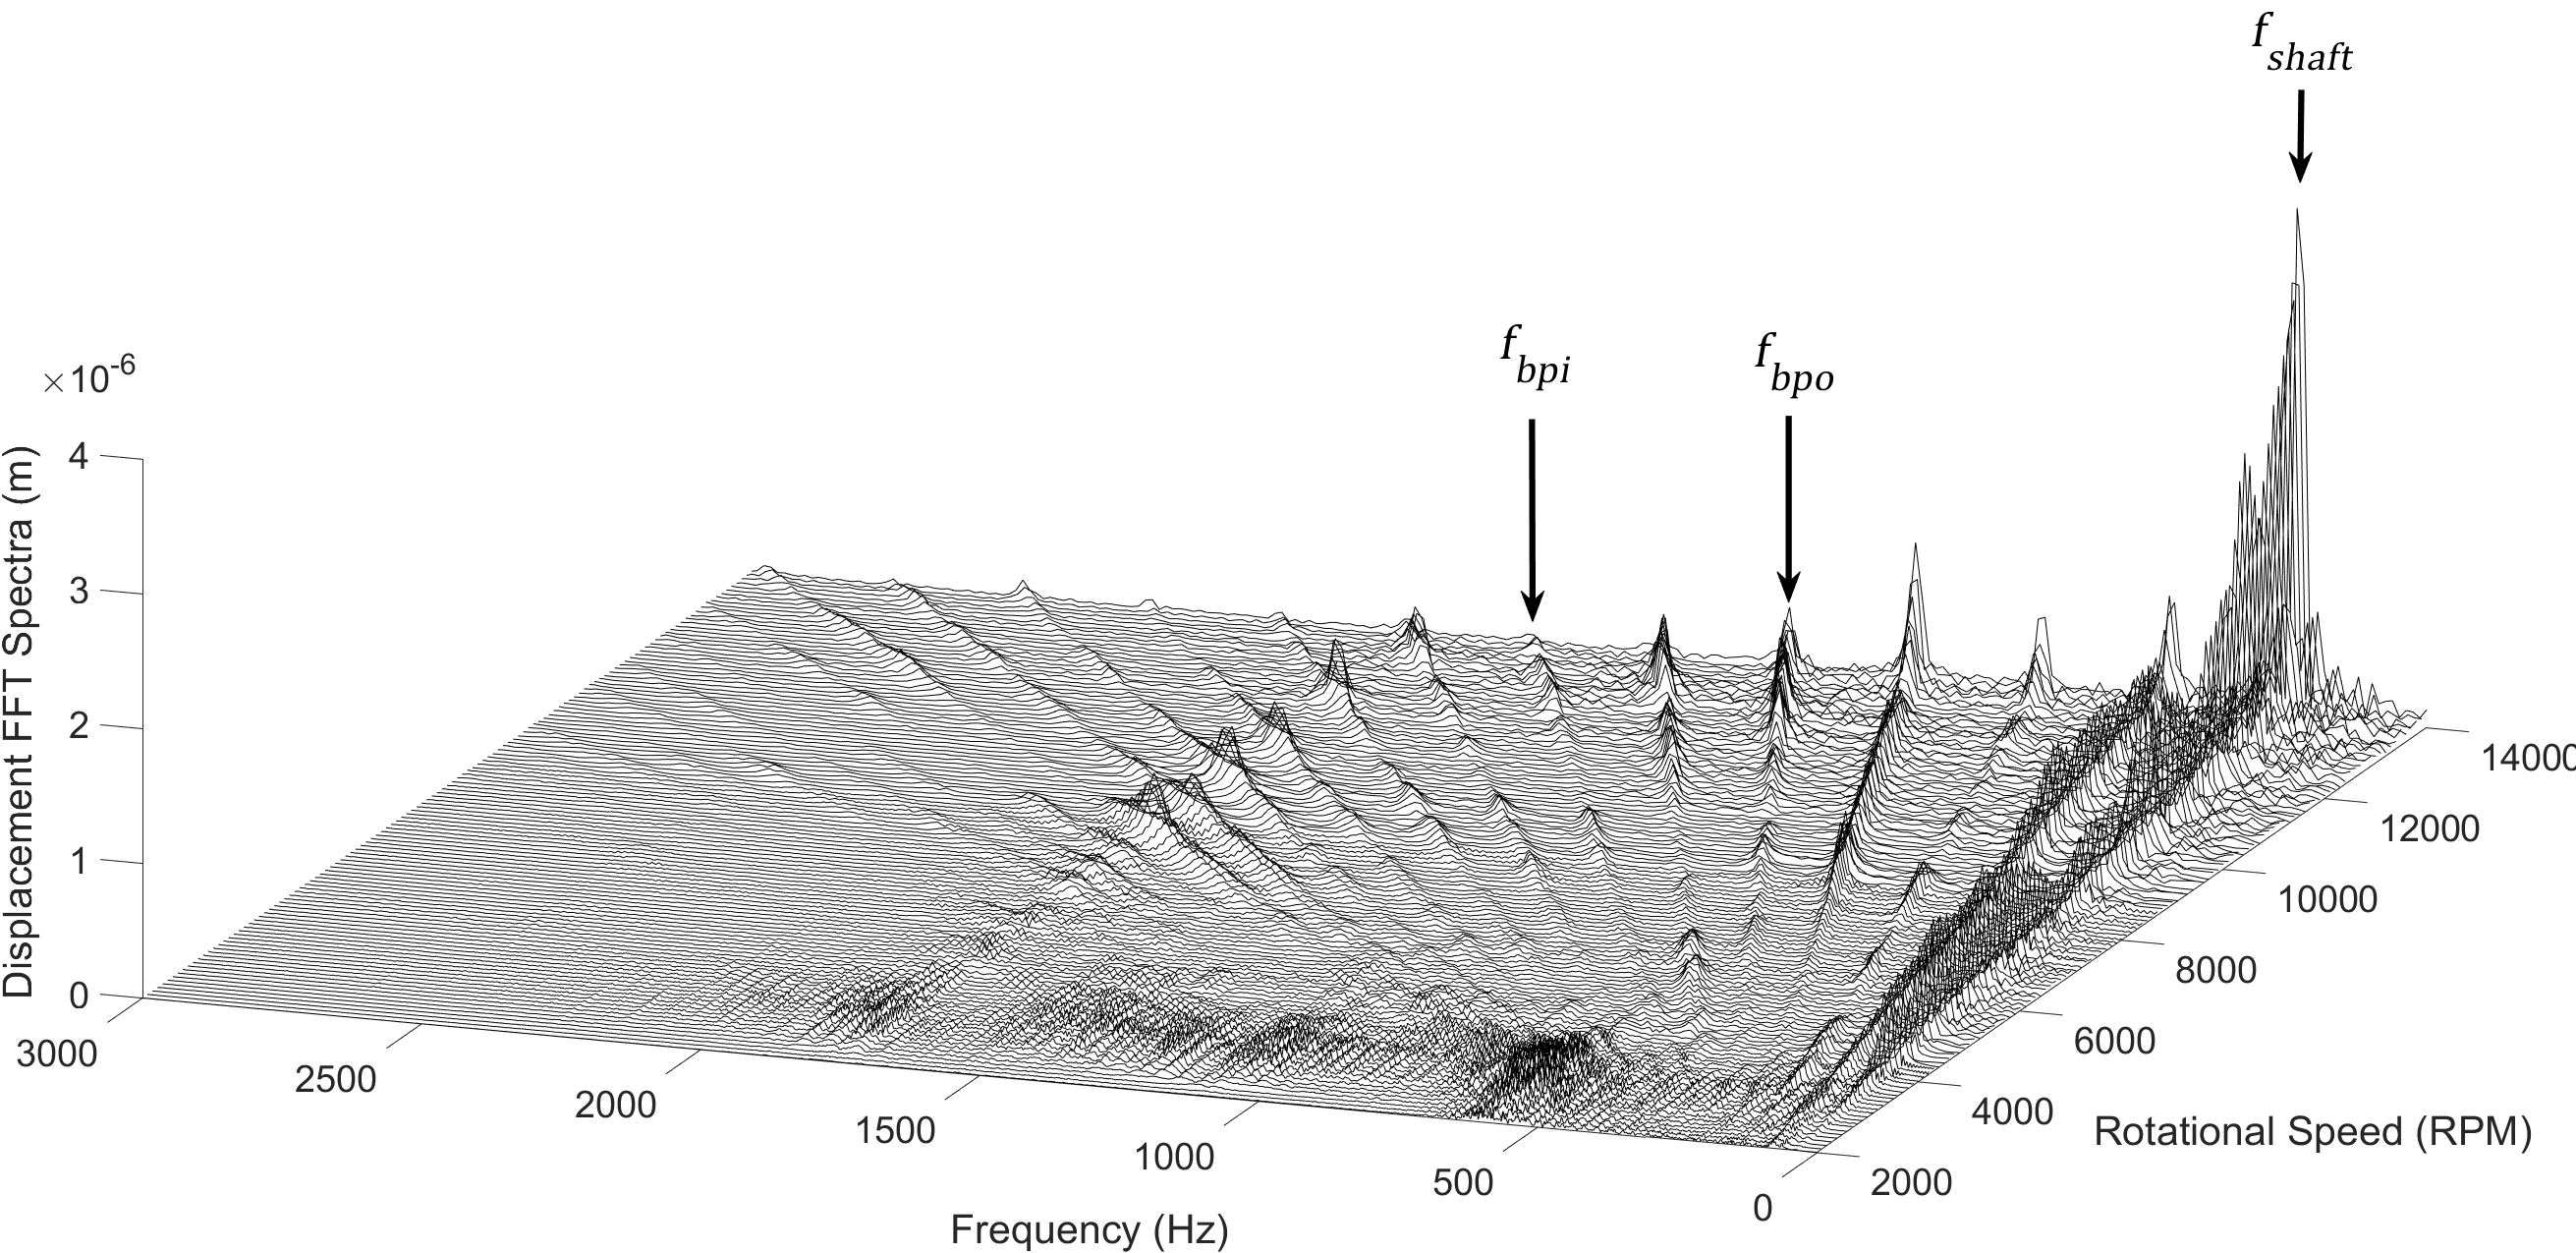
\includegraphics[width=150mm]{ExpTribo Figure 8 - Shaft Displacement Frequency Spectra.png}
	\caption{Shaft displacement frequency spectra.}
	\label{Shaft displacement frequency spectra}
\end{figure}

\section{Results and Discussion}
This section presents the results of the numerical tribological models. The kinematic data from the experimental test rig are used as the boundary conditions to the implicit and explicit models.

\subsection{Film Thickness and Load Across Speed Sweep} 
The variation in EHL film thickness and roller contact load across the speed sweep from 0~-~15~000~$rpm$ at the outer race contact are shown in Figure \ref{Contact load and film thickness - Outer race}. Only the EHL regions are shown, where loads are significant enough to cause contact deformation. The upper limit of the film is where the roller and races diverge and approach the hydrodynamic regime where the film is hence governed by the entraining motion of lubricant into the contact. The lubricant film, as seen from the film thickness equation, is more affected by the speed of entraining motion rather than the load. This explains the increasing film thickness values in Figure \ref{Contact load and film thickness - Outer race}, despite increasing load. The film thickness is increased from 0.1 to 1.9~$\mu m$ across the speed sweep, revealing a significant increase that can affect the tribodynamic behaviour of the bearing, as explained in following sections. Full system and rotor dynamics also contribute to the total load on the roller, with periods of resonance at 3~000~$rpm$ and 14~000~$rpm$, marked as $A$ and $B$ respectively in Figure \ref{Contact load and film thickness - Outer race}.

\begin{figure}
	\centering
	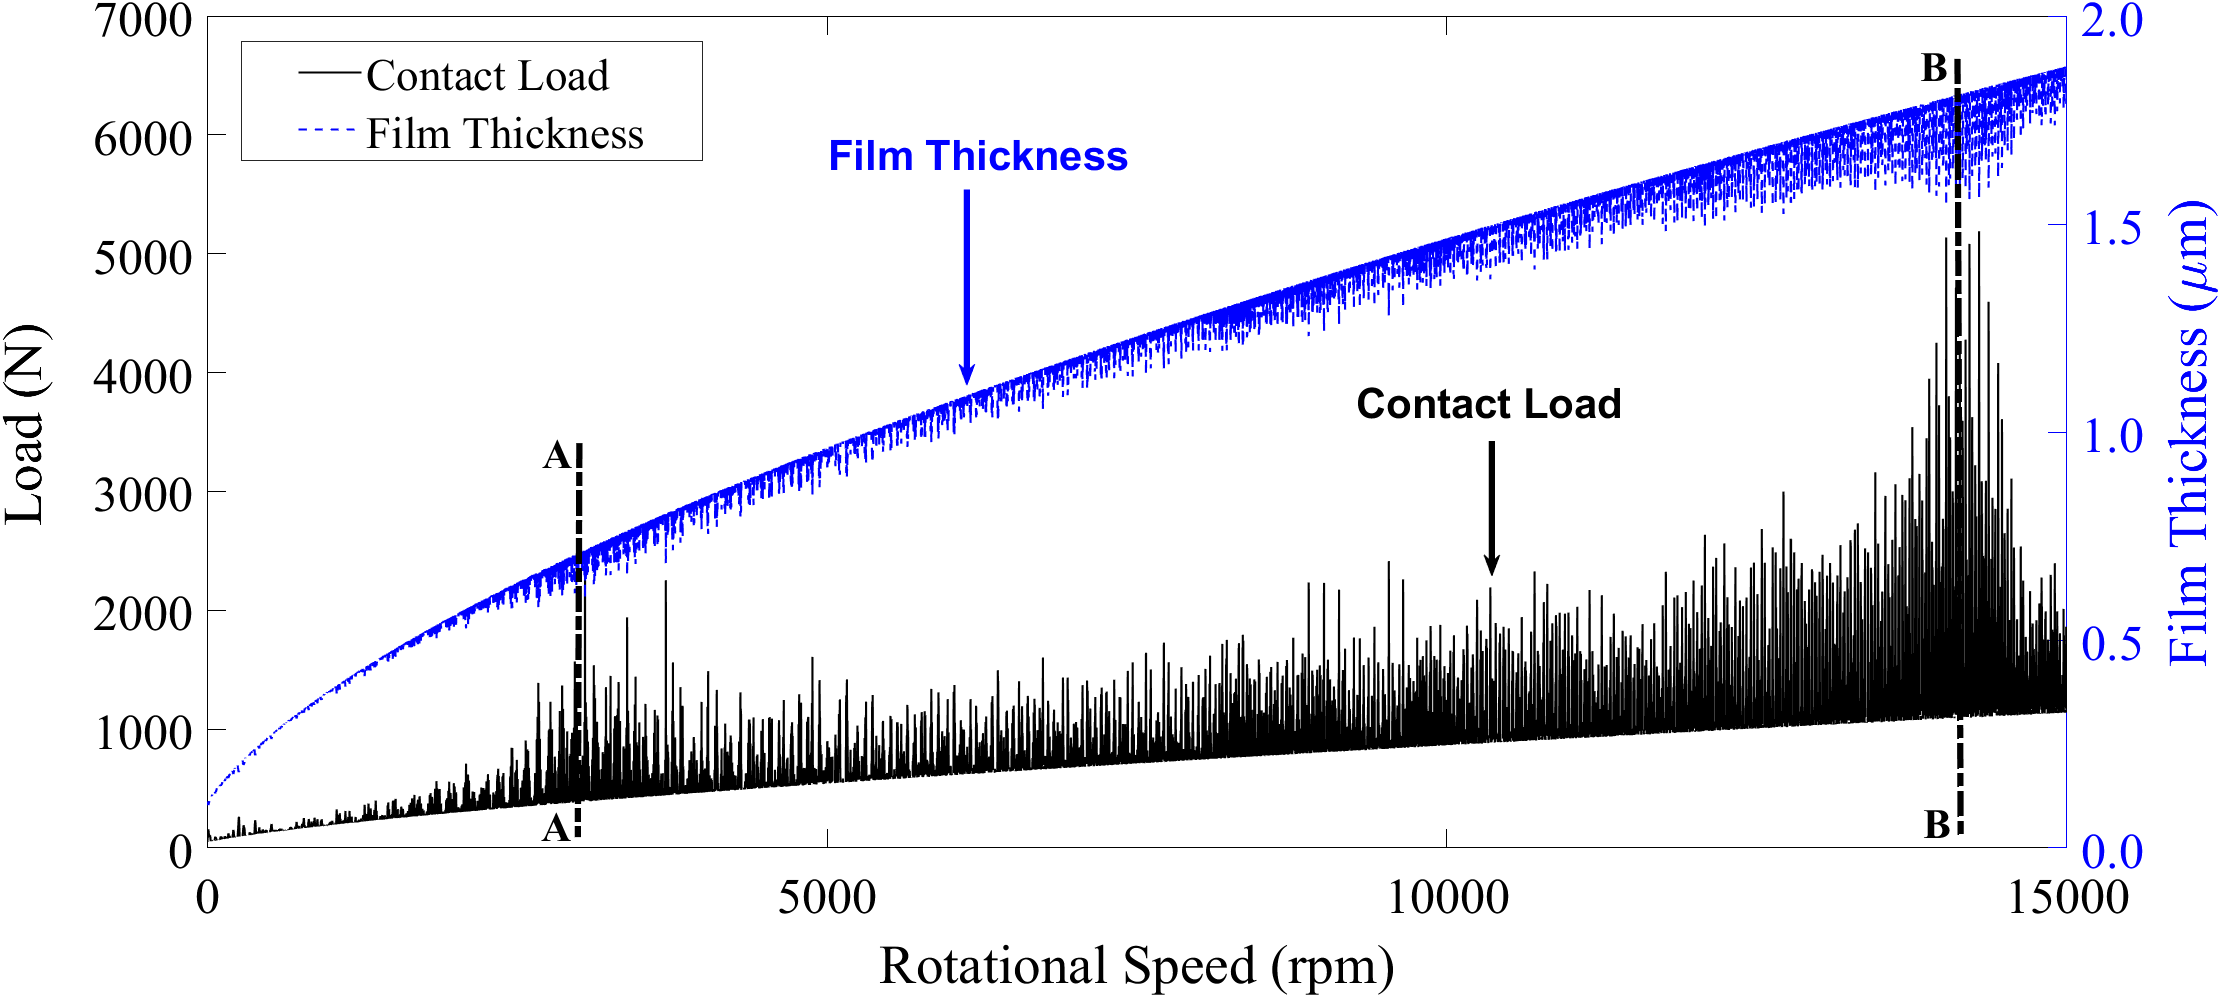
\includegraphics[width=150mm]{ExpTribo Figure 11 - Contact Load and Film Thickness - Outer Race.png}
	\caption{Contact load and film thickness - Outer race.}
	\label{Contact load and film thickness - Outer race}
\end{figure}

Figure \ref{Film and load - EHL to hydrodynamic regime} presents an interval of the speed sweep where the effect of the EHL load on reducing the film thickness under oscillating conditions can be observed and the hydrodynamic film growth as the roller is unloaded. It is possible to see the effect of the resonant frequency at 1765~$Hz$ superimposed on the lower fundamental train frequency within the loaded region as the inner and outer rings converge and diverge. The results in Figure \ref{Film and load - EHL to hydrodynamic regime} confirm the significant effect of dynamic behaviour as well as the multi-regime nature of the lubrication due to dynamic effects.

\begin{figure}
	\centering
	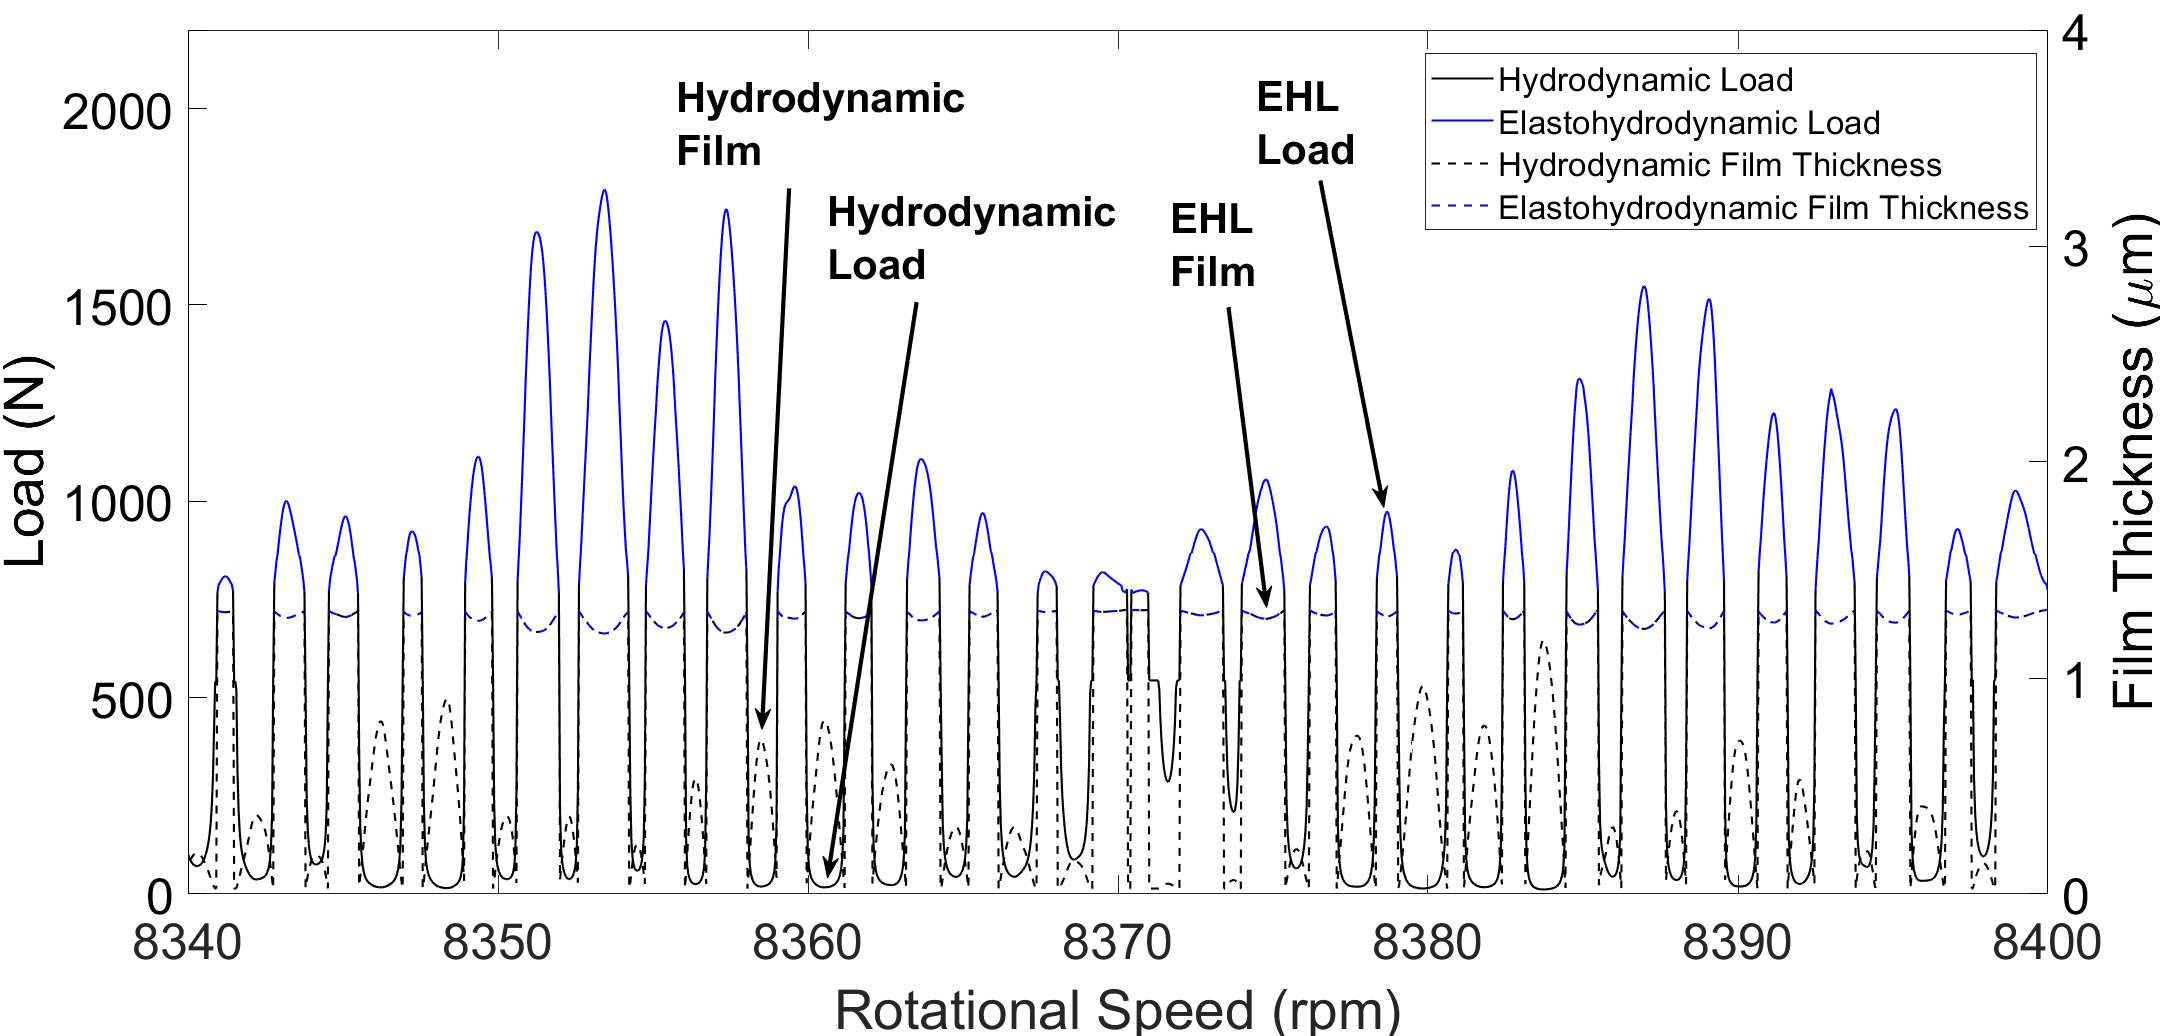
\includegraphics[width=150mm]{ExpTribo Figure 12 - Film and Load - EHL to Hydrodynamic Regime.png}
	\caption{Film and load - EHL to hydrodynamic regime.}
	\label{Film and load - EHL to hydrodynamic regime}
\end{figure} 

\subsection{EHL Regimes} \label{Greenwood EHL Regimes}

As has been demonstrated in the results analysis, the contact conditions deviate from the elastohydrodynamic regime of lubrication into the hydrodynamic regime throughout the roller orbital motion. These conditions can be verified by presenting the results on the Greenwood chart for fluid regimes of lubrication. The charts display the physical effects instrumental to EHL formation under isothermal conditions: viscosity rise due to pressure and elastic deformation of the surface. These two effects are quantified by two dimensionless parameters, $G_e$ and $G_v$, as defined below \cite{Gohar1988}: 

\begin{equation}\label{GoharGe}
	G_e=\frac{W^*}{U^{* 1 / 2}}
\end{equation}

\begin{equation}\label{GoharGv}
	G_v=\frac{W^{* 3 / 2} G^*}{U^{* 1 / 2}}
\end{equation}

Four regions exist and the boundaries of these regions are defined by the geometry of contacting bodies, material, and lubricant properties. As is shown in Figure \ref{EHL and hydrodynamic conditions during roller operation}, the outer roller-race contact conditions move between the viscous elastic (VE) and iso-viscous rigid (IR) regimes. The VE regime signifies the EHL regime of lubrication where contact pressures are such that the elastic deformation of the surfaces and viscosity rise due to pressure increase is significant. The IR regime occurs when the magnitude of elastic deformation is insignificant, and the contact pressures are low enough that viscosity rise is negligible, i.e. hydrodynamic lubrication \cite{Hamrock1980}. The boundary between the two also corresponds well with the distinction being made between hydrodynamic and EHL in this methodology, presented by the black and blue regions of the plot.

\begin{figure}
	\centering
	\includegraphics[width=150mm]{ExpTribo Figure 14 – EHL and hydrodynamic conditions during roller operation.png}
	\caption{EHL and hydrodynamic conditions during roller operation. Key: IR = Iso-viscous Rigid, VR = Viscous Rigid, VE = Viscous Elastic, IE = Iso-viscous Elastic.}
	\label{EHL and hydrodynamic conditions during roller operation}
\end{figure} 

\subsection{Dry vs Lubricated Tribodynamic Model}

Previously presented results confirmed the significance of considering tribodynamic coupling on the tribological predictions. The aim of this section is to assess the significance of this coupling on dynamics via affecting contact load and stiffness values. The surface deformation at the EHL contact is further exacerbated by the presence of the lubricant film. Since the contact load and contact stiffness are governed by this deformation, neglecting the film leads to an underestimation of the total load at the roller-race contact. At higher speeds, such as those present in modern electrified powertrains, the growth of the lubricant film due to the increased entraining motion into the conjunction cannot be neglected – as is shown in Figure \ref{Contact load and film thickness - Outer race} with a film growth from 0.1 to 1.9~$\mu m$. The implicit tribological model was run for two cases, including and negating lubricant film thickness in the deformation obtained from Equation \ref{Contact deflection experimental}. The difference in magnitude at each time step is computed, and the increase in load magnitude between a dry and lubricated model is calculated. For EHL loads, the magnitude of the load difference through the speed sweep is plotted in Figure \ref{Contact load difference between dry and lubricated model}.

\begin{figure}
	\centering
	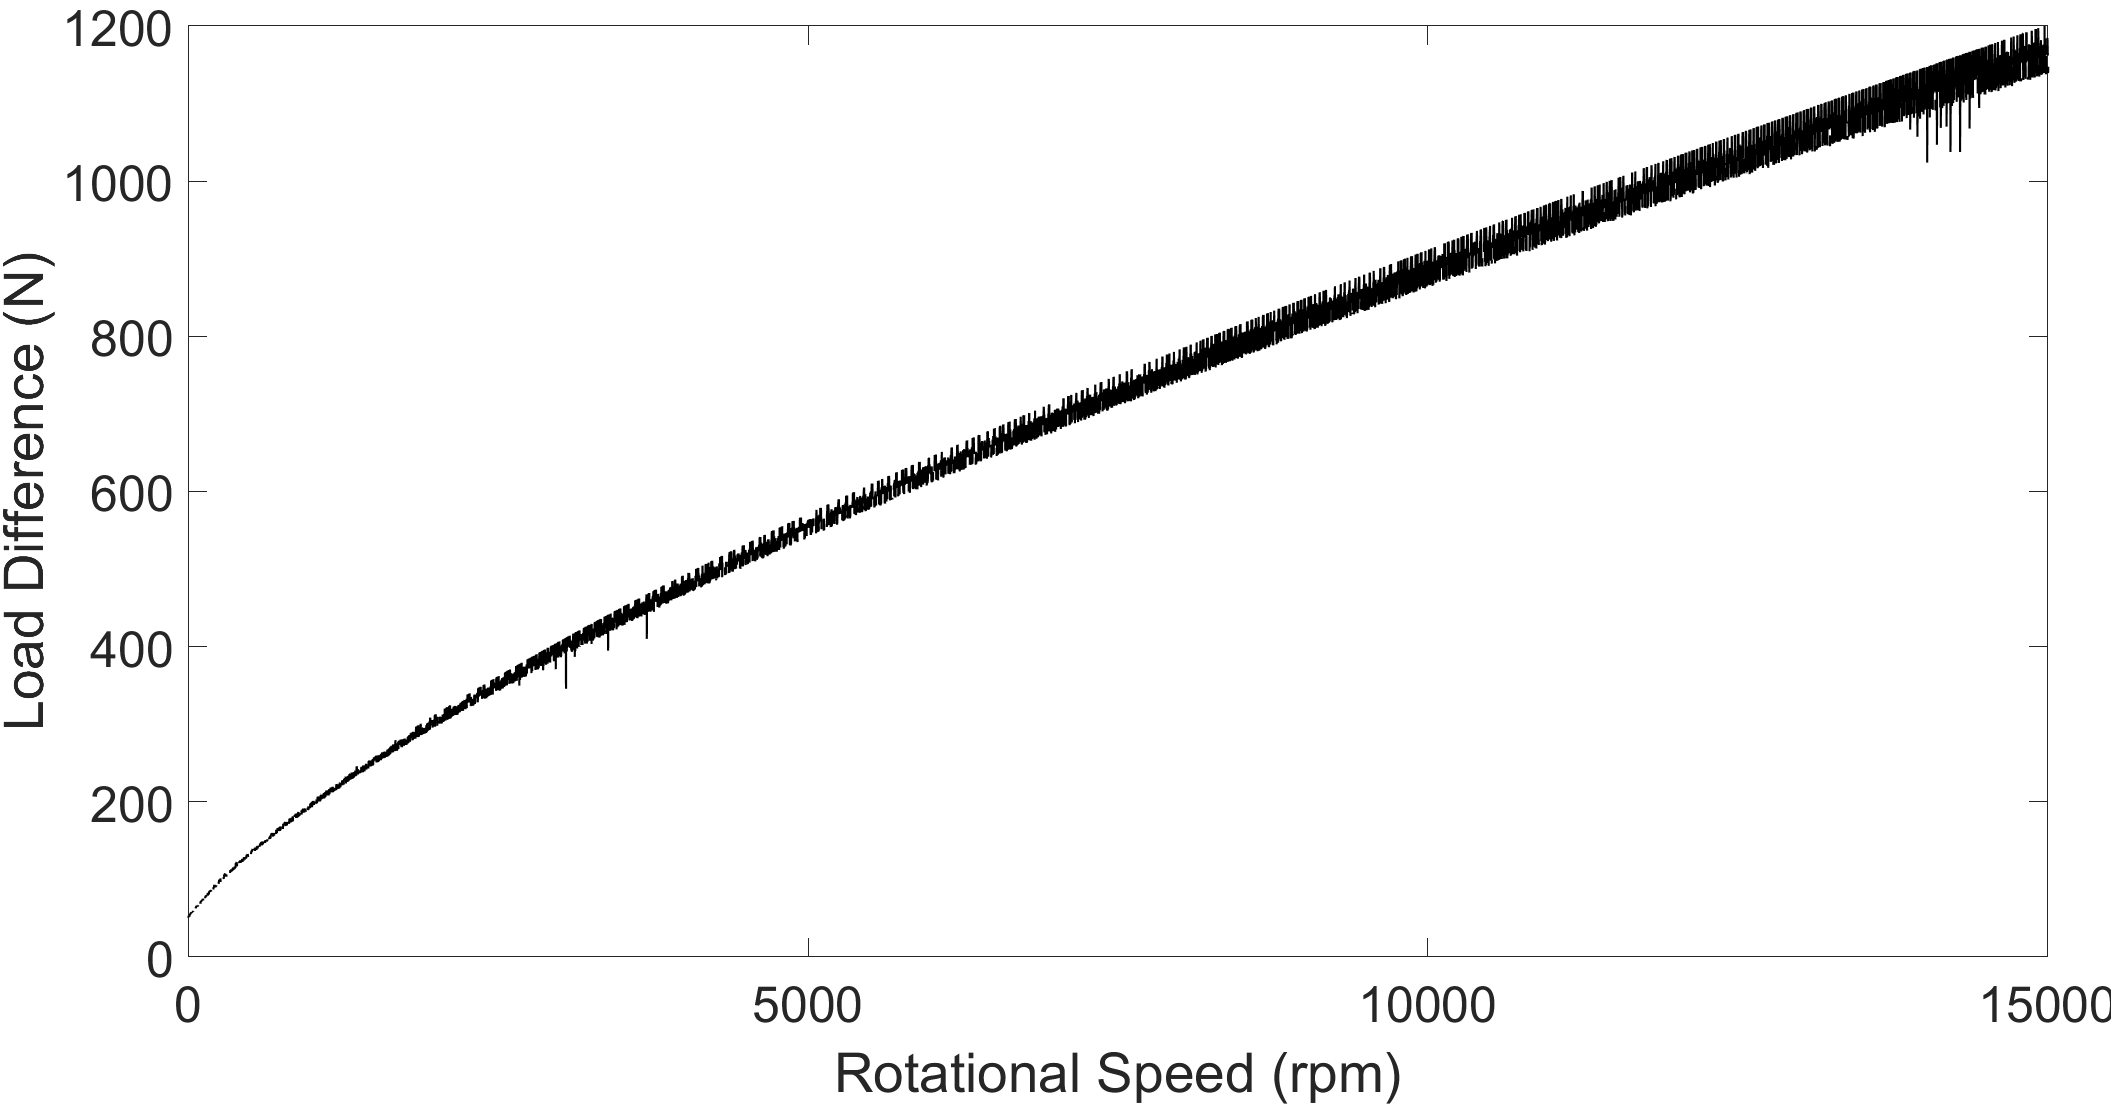
\includegraphics[width=150mm]{ExpTribo Figure 15 - Contact Load Difference Between Dry and Lubricated Model.png}
	\caption{Contact load difference between dry and lubricated model.}
	\label{Contact load difference between dry and lubricated model}
\end{figure} 

There is an increasing contact load difference across the speed sweep, with fluctuations arising from the dynamics of the system. To fully understand the requirement for a lubricated bearing model, the percentage difference between both cases is presented at three different rotational speed snapshots of 3~050~$rpm$, 14~135~$rpm$, and 14~855~$rpm$ in Figure \ref{Dry and lubricated model load difference}. At low speeds and relatively low dynamic load, the addition of the film contributes to a 14.8\% greater load prediction than a dry model, showing that the film inclusion has a significant contribution even at low rotational speeds. At shaft speeds of 14~135~$rpm$, the first order resonance in the system, as shown in the frequency plots, creates high dynamic loading. At peak load, the growth of the film is still present, however, the high contact deformation is close to the magnitude of the film growth, hence the difference between dry and lubricated model reaches 25.1\%. As the system passes through this resonant region and the overall dynamic load is reduced, the percentage load difference reaches values as high as 149\% as the effect of the film growth at high speeds exceeds that of the surface deformation.

\begin{figure}
	\centering
	\begin{subfigure}{0.75\textwidth}
		\centering
		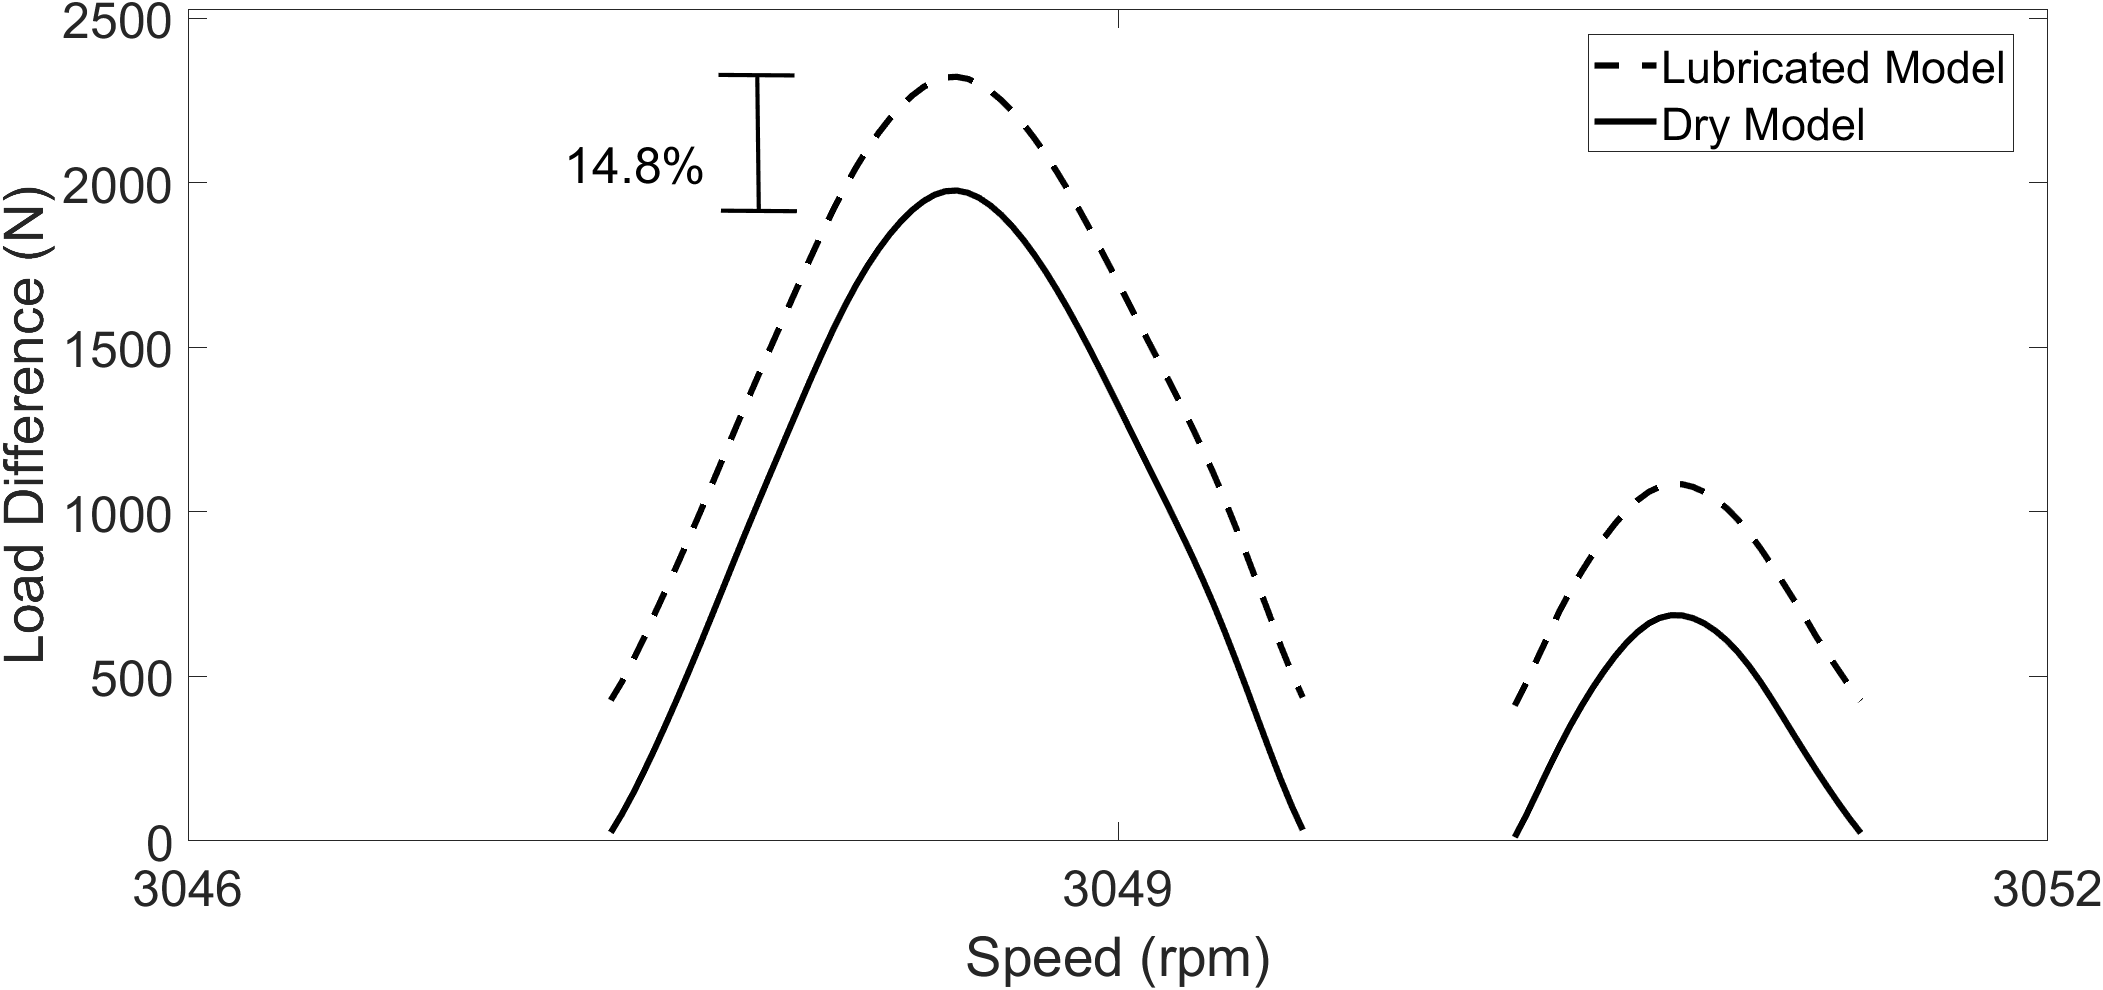
\includegraphics[width=\textwidth]{ExpTribo Figure 16a.png}
		\caption{}
		\label{3050rpm}
	\end{subfigure}
	\hfill
	\begin{subfigure}{0.75\textwidth}
		\centering
		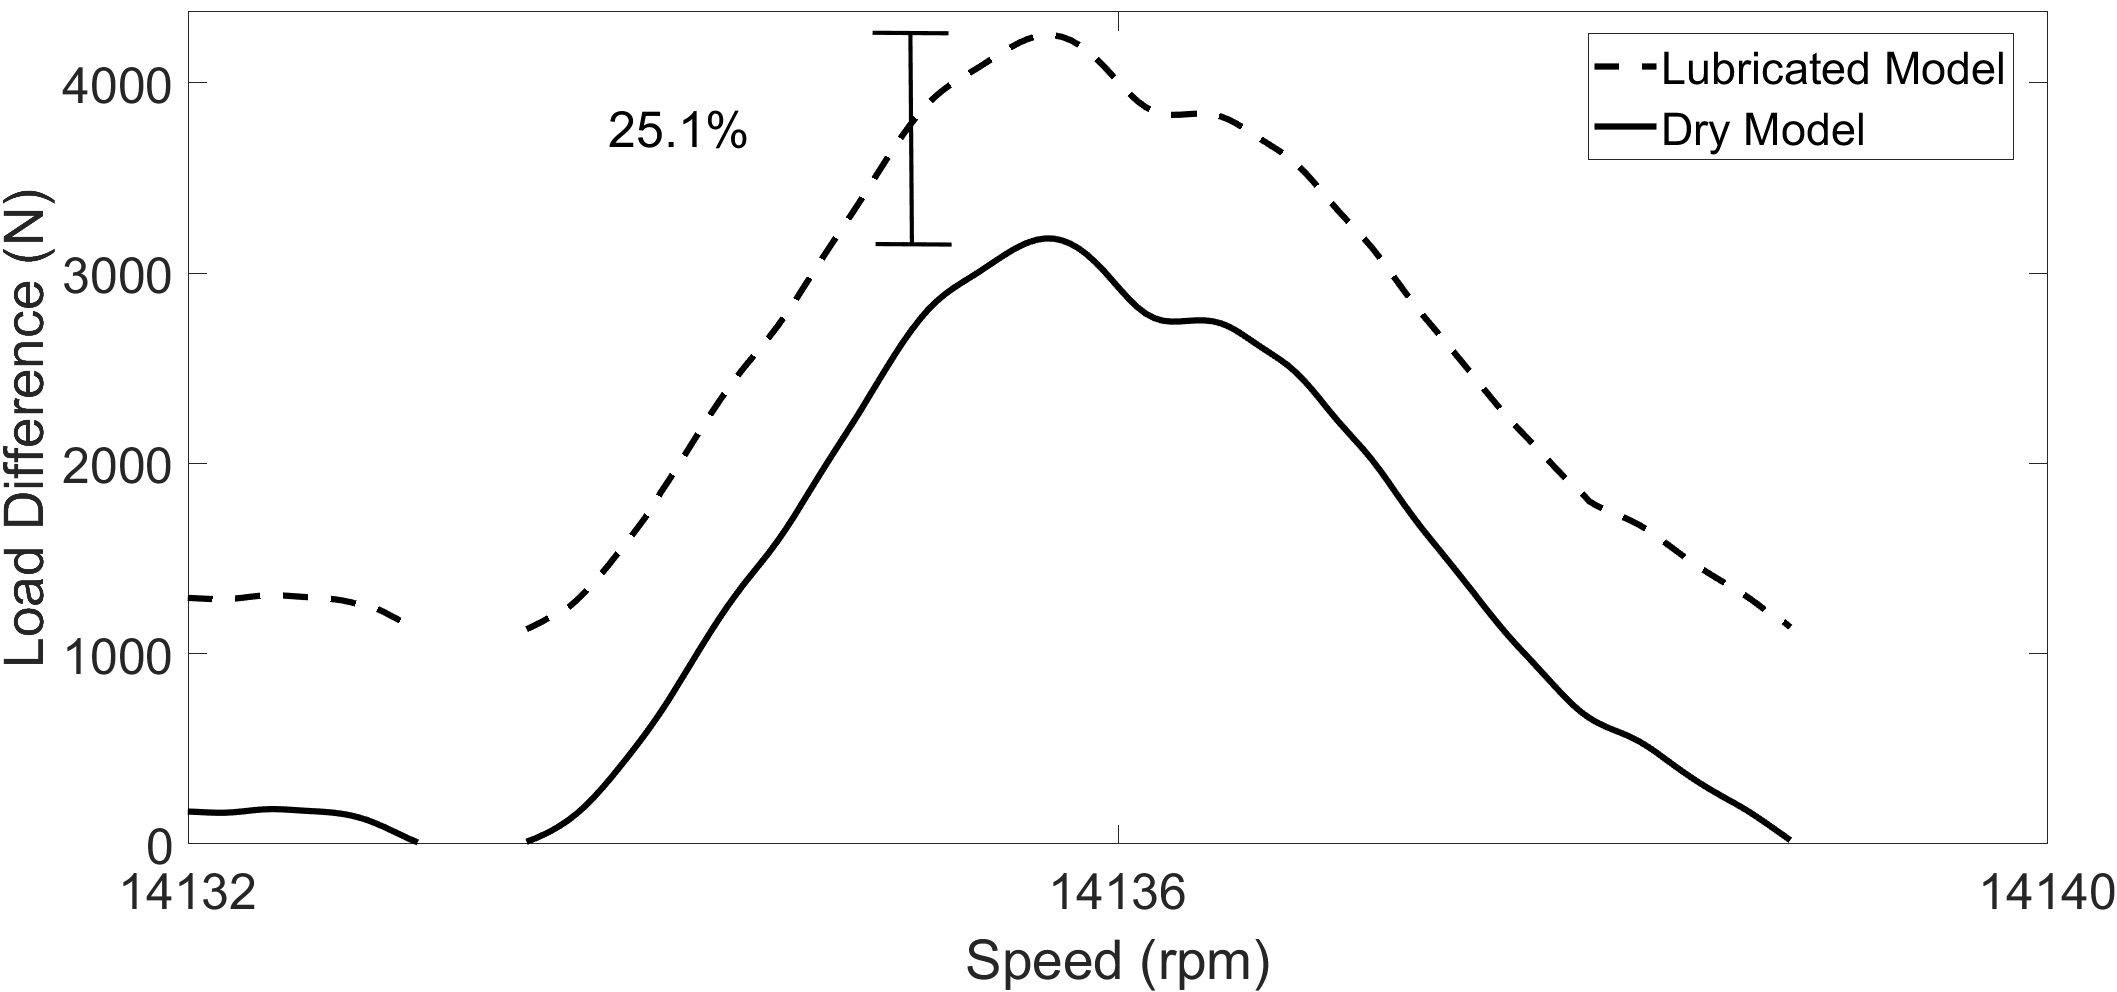
\includegraphics[width=\textwidth]{ExpTribo Figure 16b.png}
		\caption{}
		\label{14135rpm}
	\end{subfigure}
	\vfill
	\begin{subfigure}{0.75\textwidth}
		\centering
		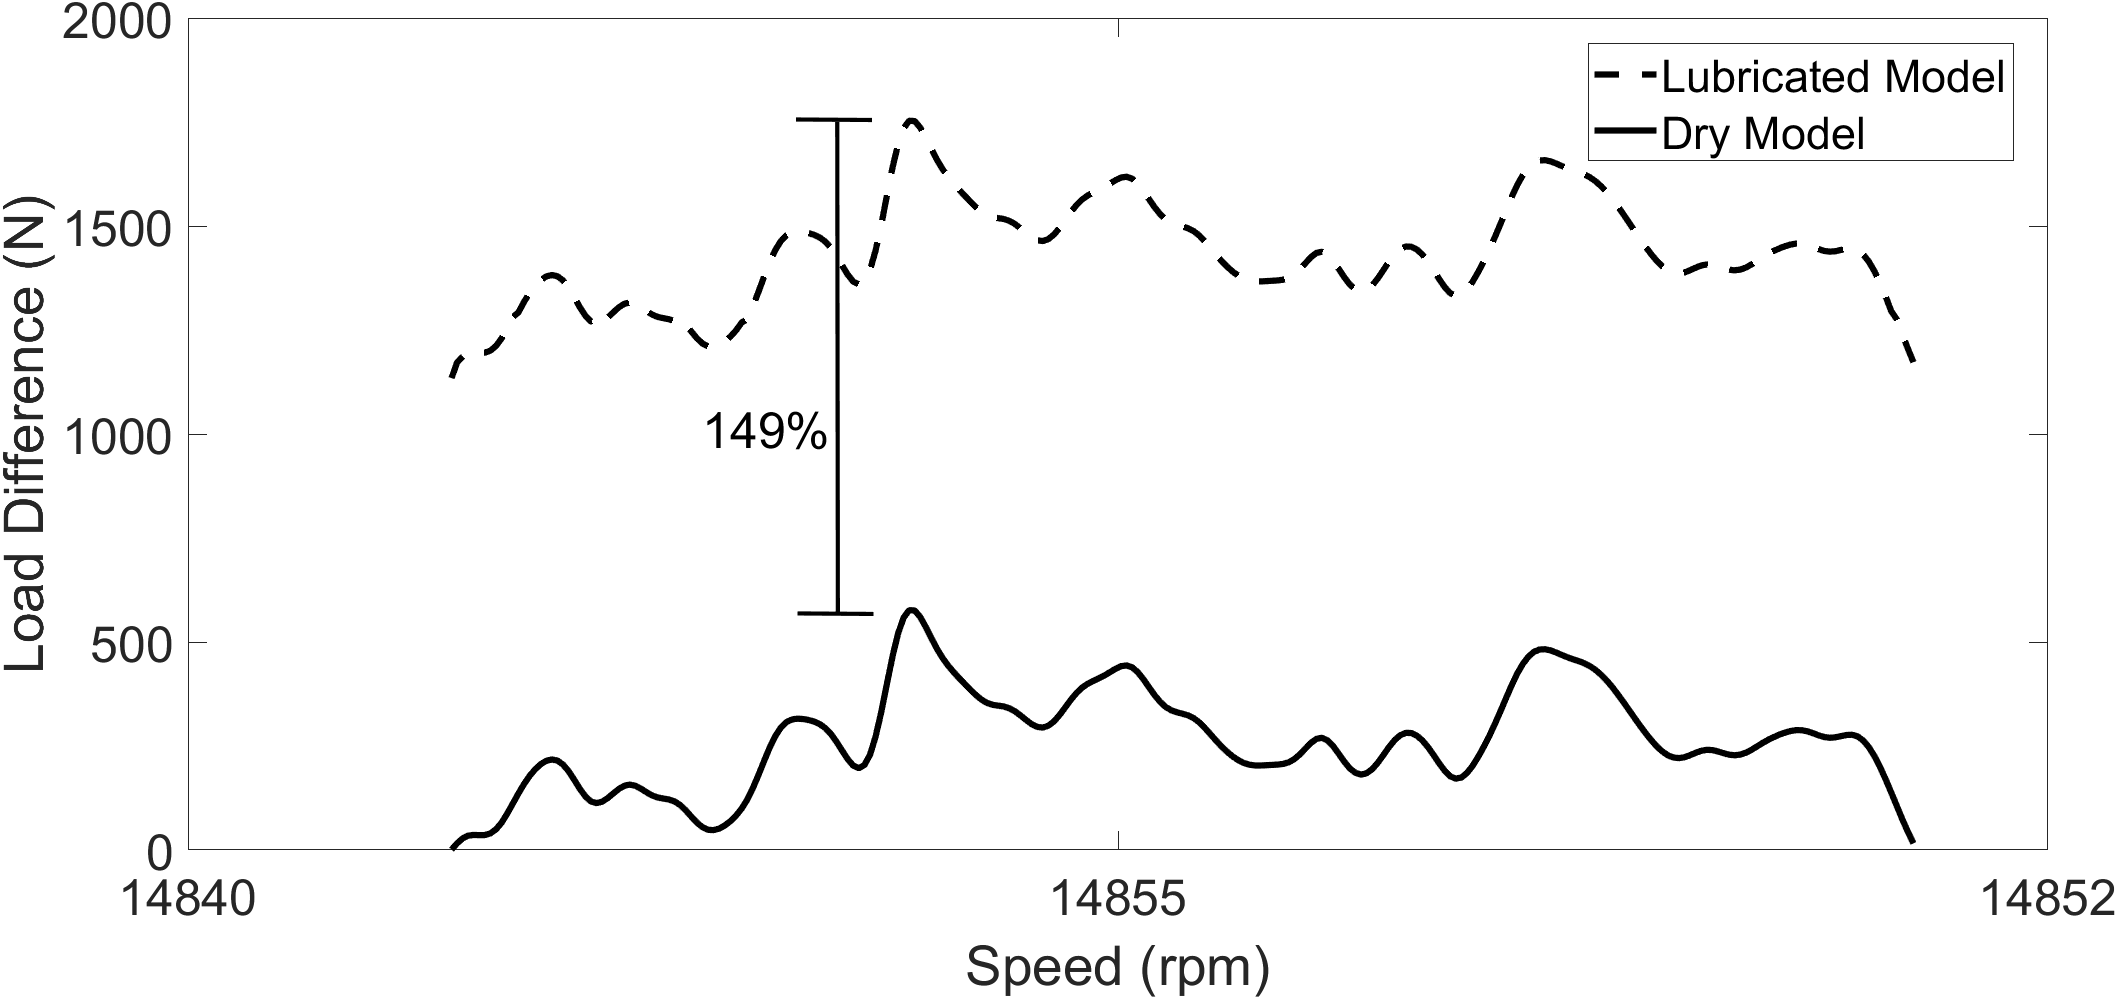
\includegraphics[width=\textwidth]{ExpTribo Figure 16c.png}
		\caption{}
		\label{14855rpm}
	\end{subfigure}
	\caption{Dry and lubricated model load difference: a) 3~050~$rpm$, b) 14~135~$rpm$, c) 14~855~$rpm$.}
	\label{Dry and lubricated model load difference}
\end{figure}

At high speeds in periods of resonance, the magnitude of the bearing load dominates, and the effect of the increasing film thickness with speed diminishes in regions of resonance. The percentage difference between the dry and lubricated model is lower as the external force and corresponding surface deformation prevails the effect of the film. However, at high speeds outside of this period of resonance, the film thickness is of the same order as the deformation and the percentage difference between the two models is much greater.  

\subsection{Numerical EHL Results} \label{Numerical vs analytical experimental}

Full numerical simulation is required to obtain detailed pressure and film thickness distributions. These distributions reveal the realistic pressure and film values at the contact for in-depth durability, efficiency and thermal analysis. At 8~350~rpm, focussing on one roller orbit, the selected points for EHL numerical analysis are shown in Figure \ref{Selected points for the numerical EHL model}. These load values are found from the implicit tribological model when the roller enters the loaded region of the bearing. The corresponding points on the bearing circumference are also shown. 

\begin{figure}
	\centering
	\includegraphics[width=150mm]{ExpTribo Figure 17 – Selected Points for Numerical EHL Model.png}
	\caption{Selected points for the numerical EHL model.}
	\label{Selected points for the numerical EHL model}
\end{figure} 

The load values are passed explicitly to the numerical EHL model along with entrainment velocity, lubricant and solid properties. From the nodes presented, the pressure distribution and film thickness across the contact are obtained. These are presented in Figure 18.

\begin{figure}
	\centering
	\begin{subfigure}[b]{0.49\textwidth}
		\centering
		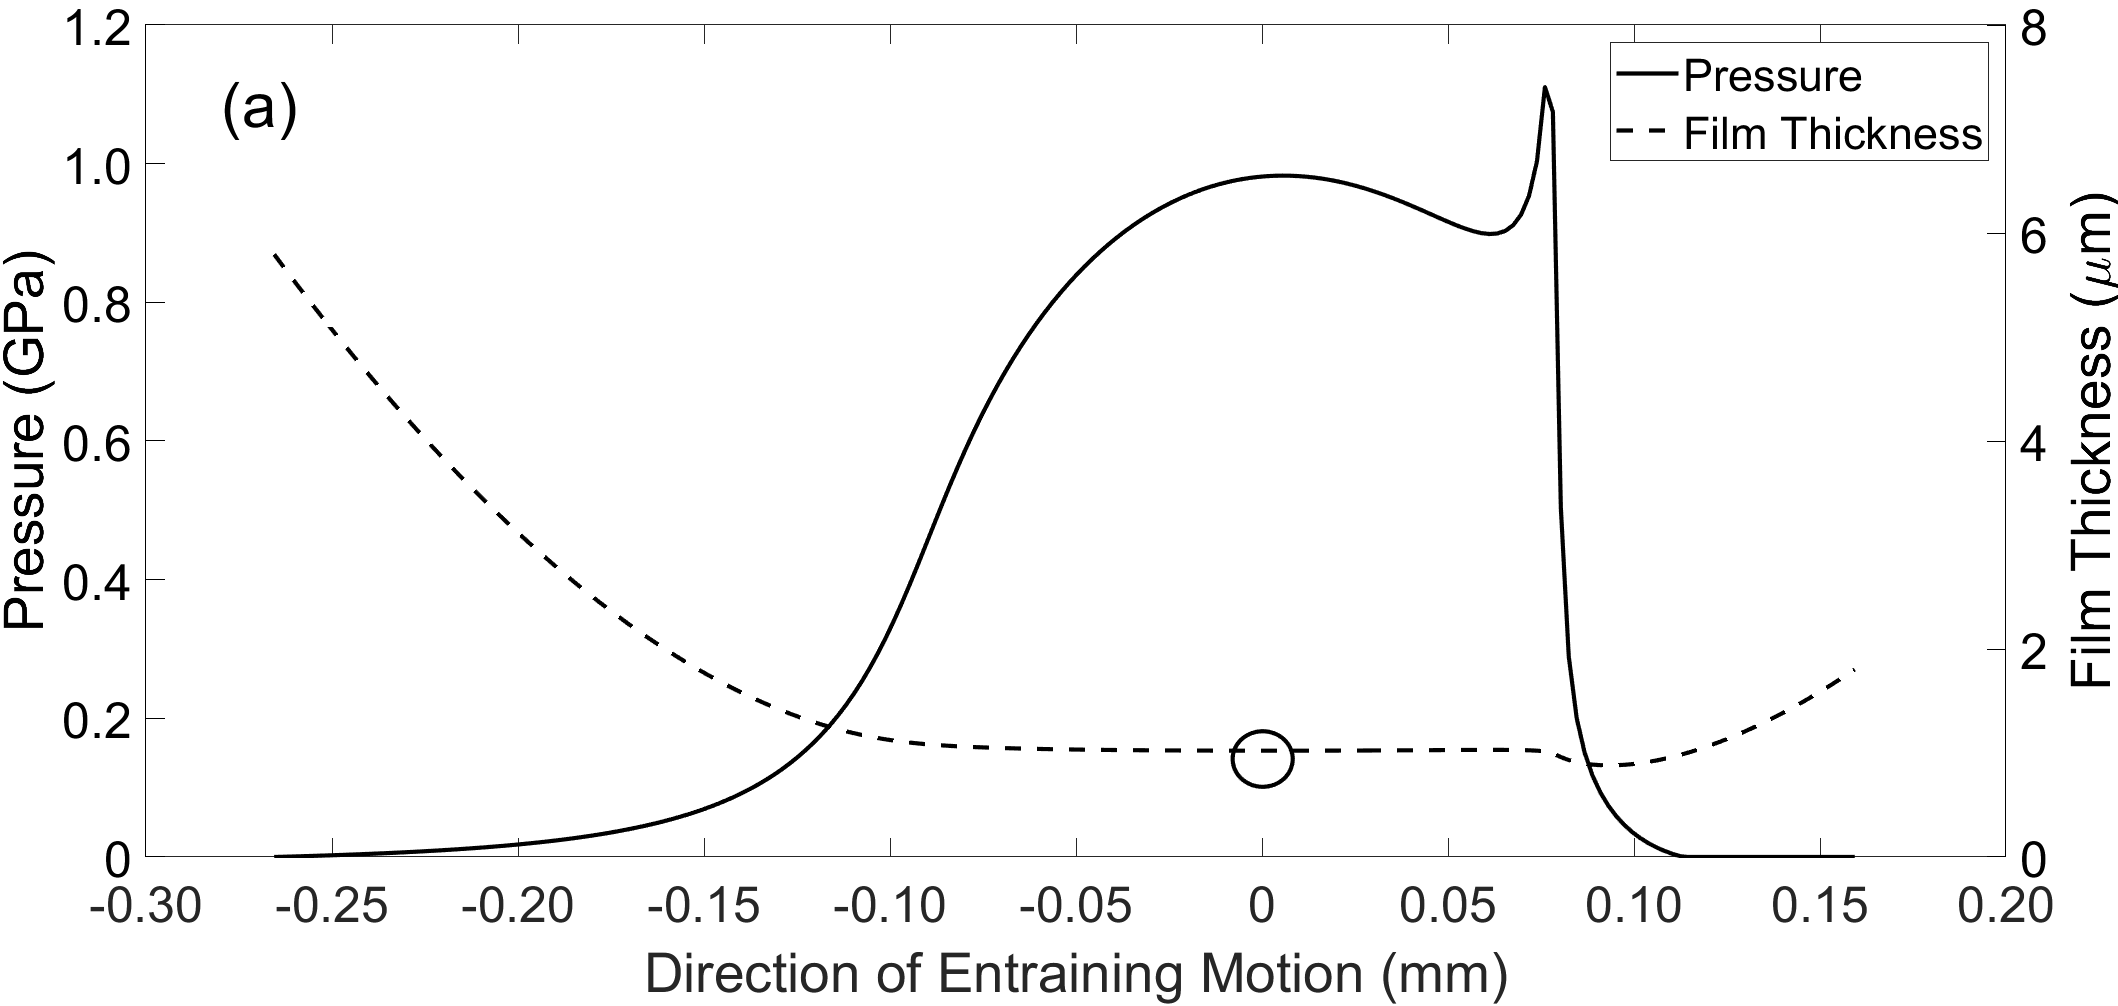
\includegraphics[width=\textwidth]{ExpTribo Figure 18a.png}
		\caption{}
		\label{NodeA}
	\end{subfigure}
	\hfill
	\begin{subfigure}[b]{0.49\textwidth}
		\centering
		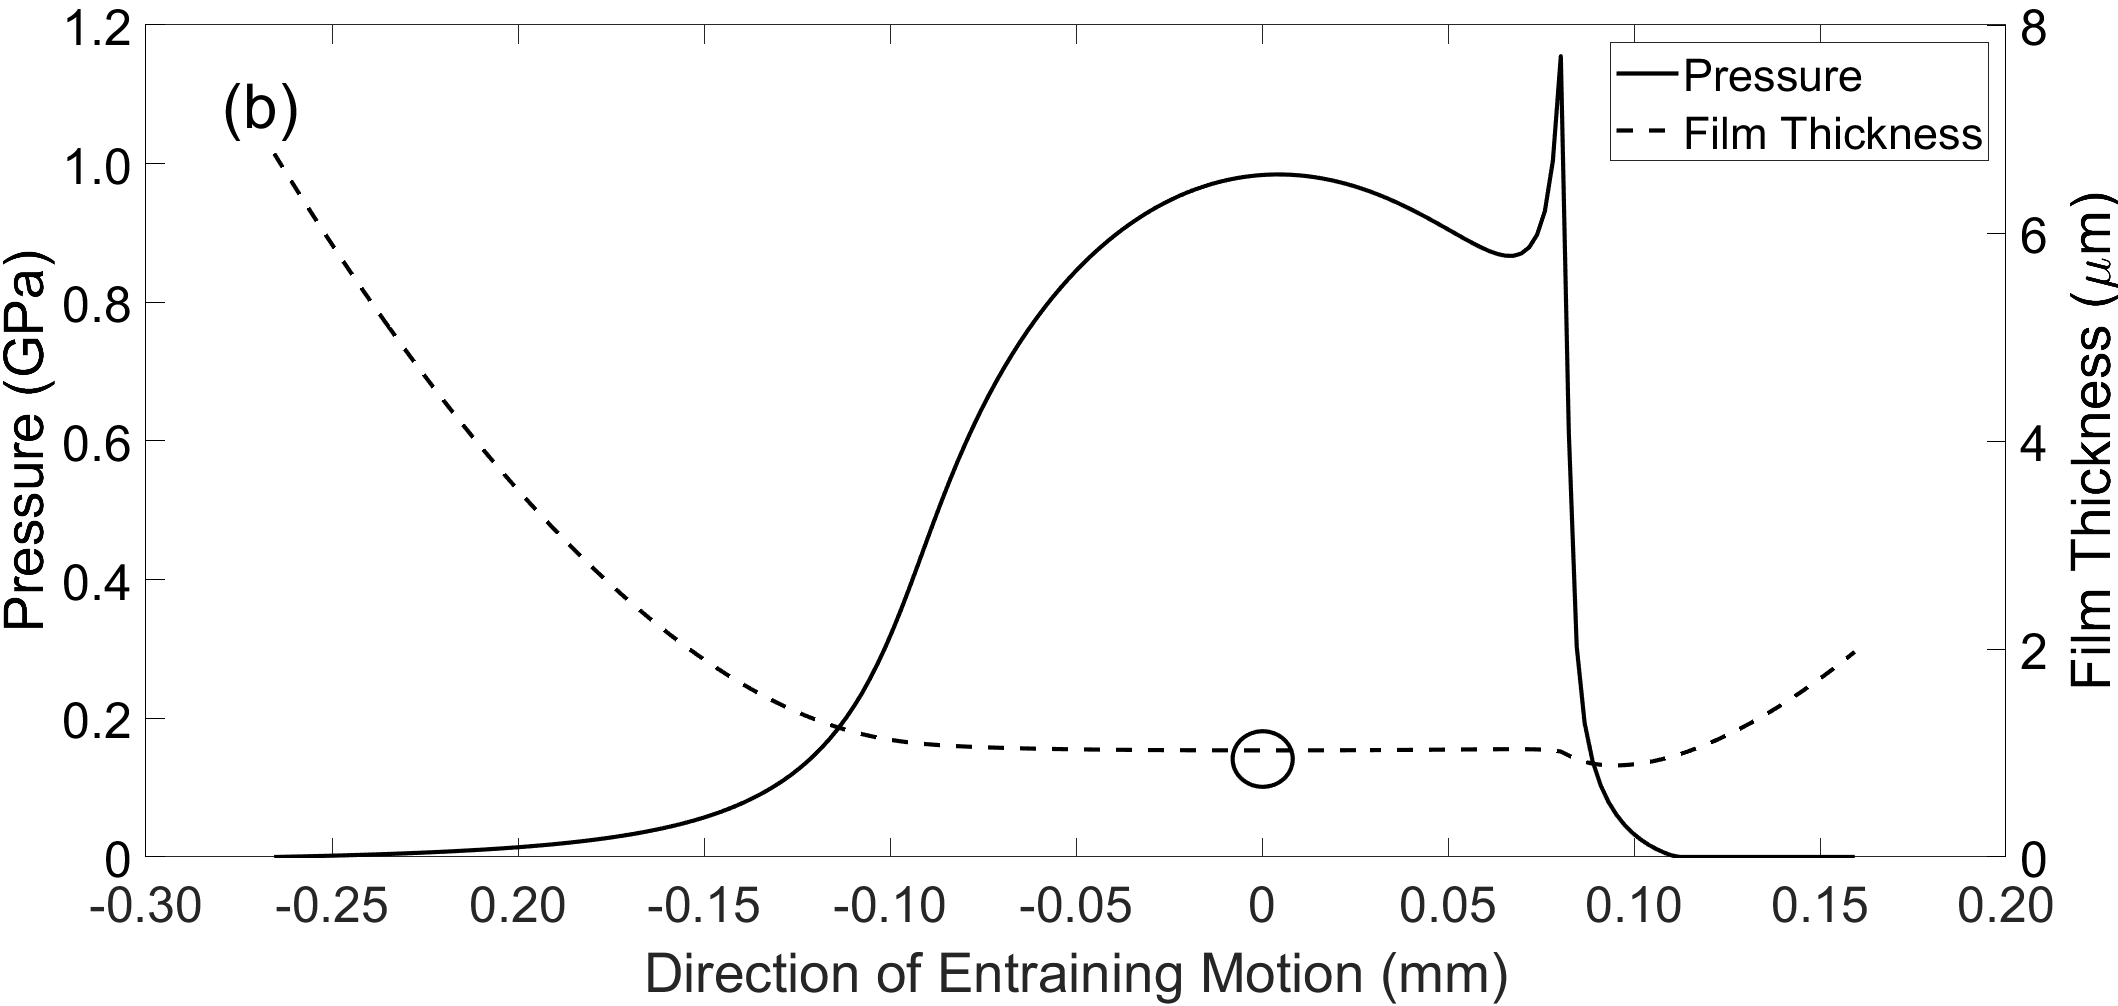
\includegraphics[width=\textwidth]{ExpTribo Figure 18b.png}
		\caption{}
		\label{NodeB}
	\end{subfigure}
	\hfill
	\begin{subfigure}[b]{0.49\textwidth}
		\centering
		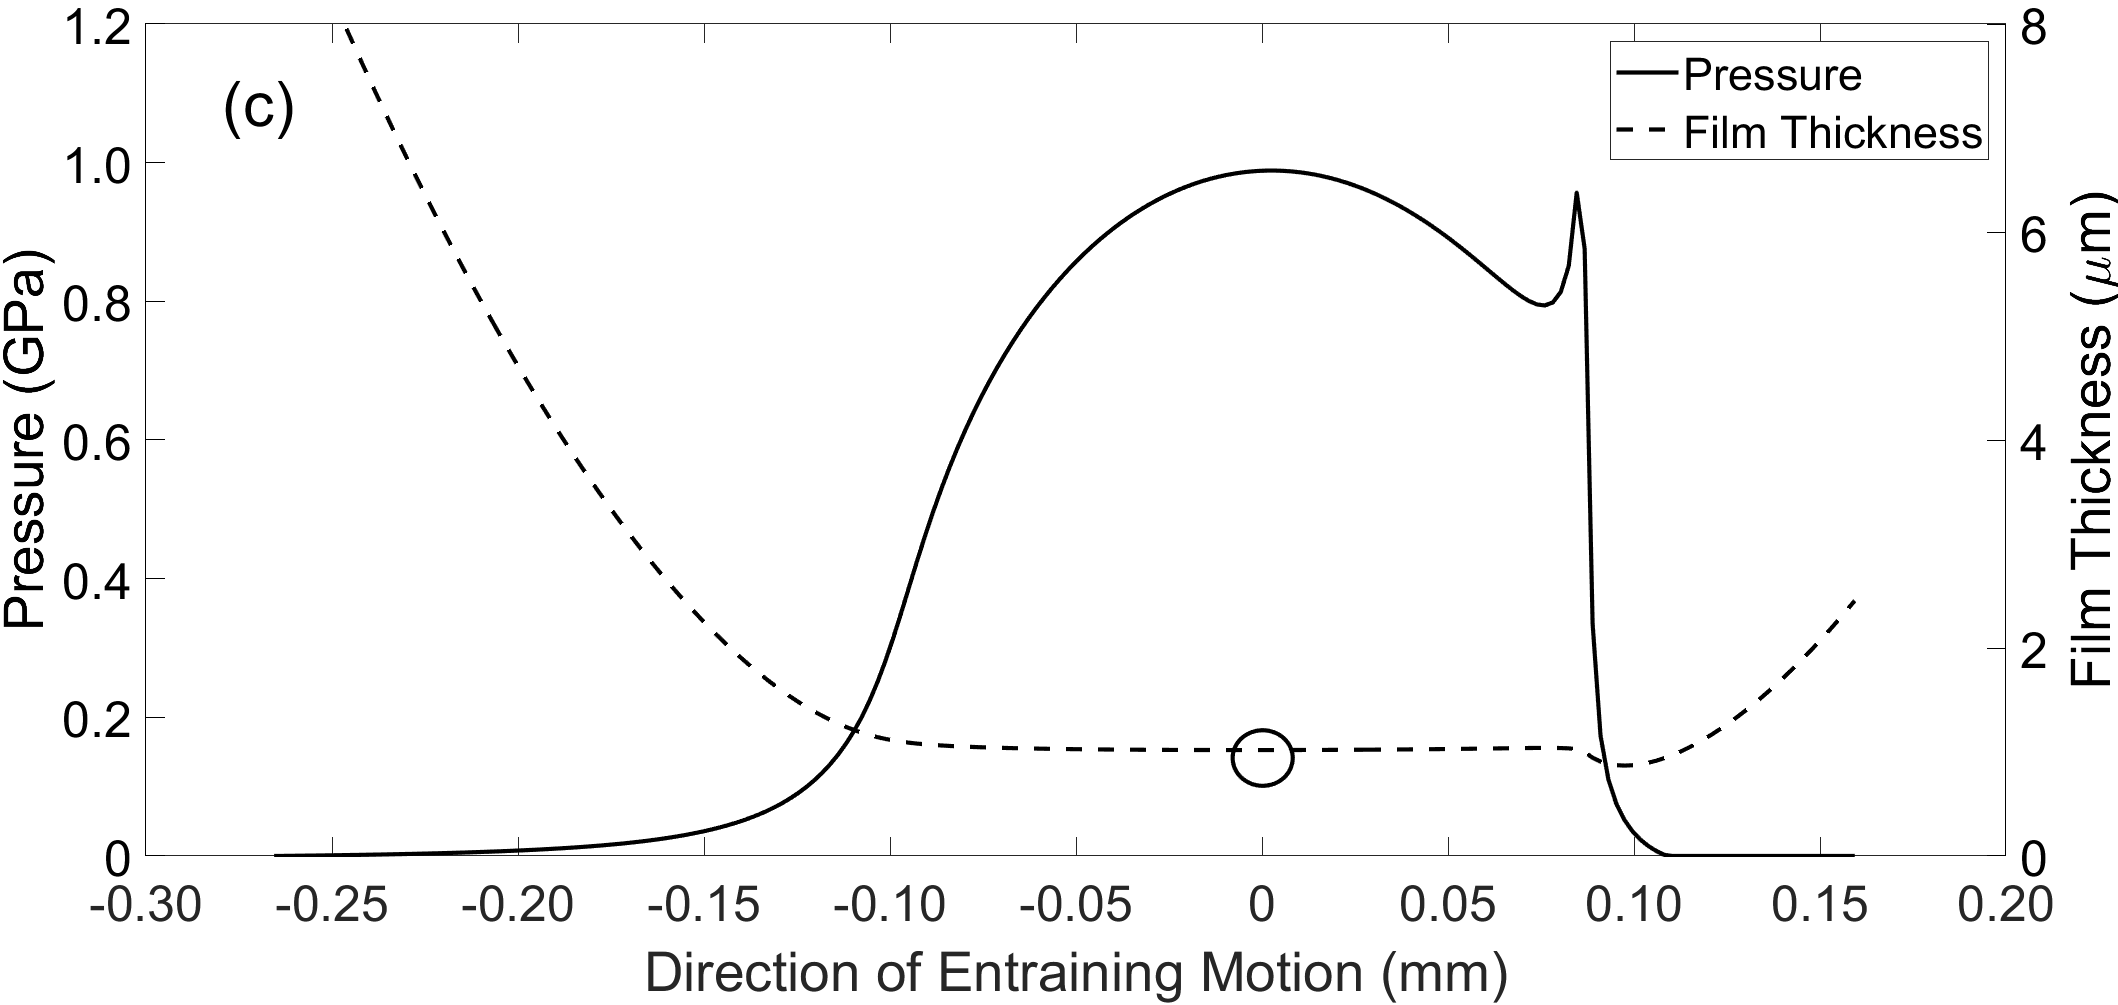
\includegraphics[width=\textwidth]{ExpTribo Figure 18c.png}
		\caption{}
		\label{NodeC}
	\end{subfigure}
	\hfill
	\begin{subfigure}[b]{0.49\textwidth}
		\centering
		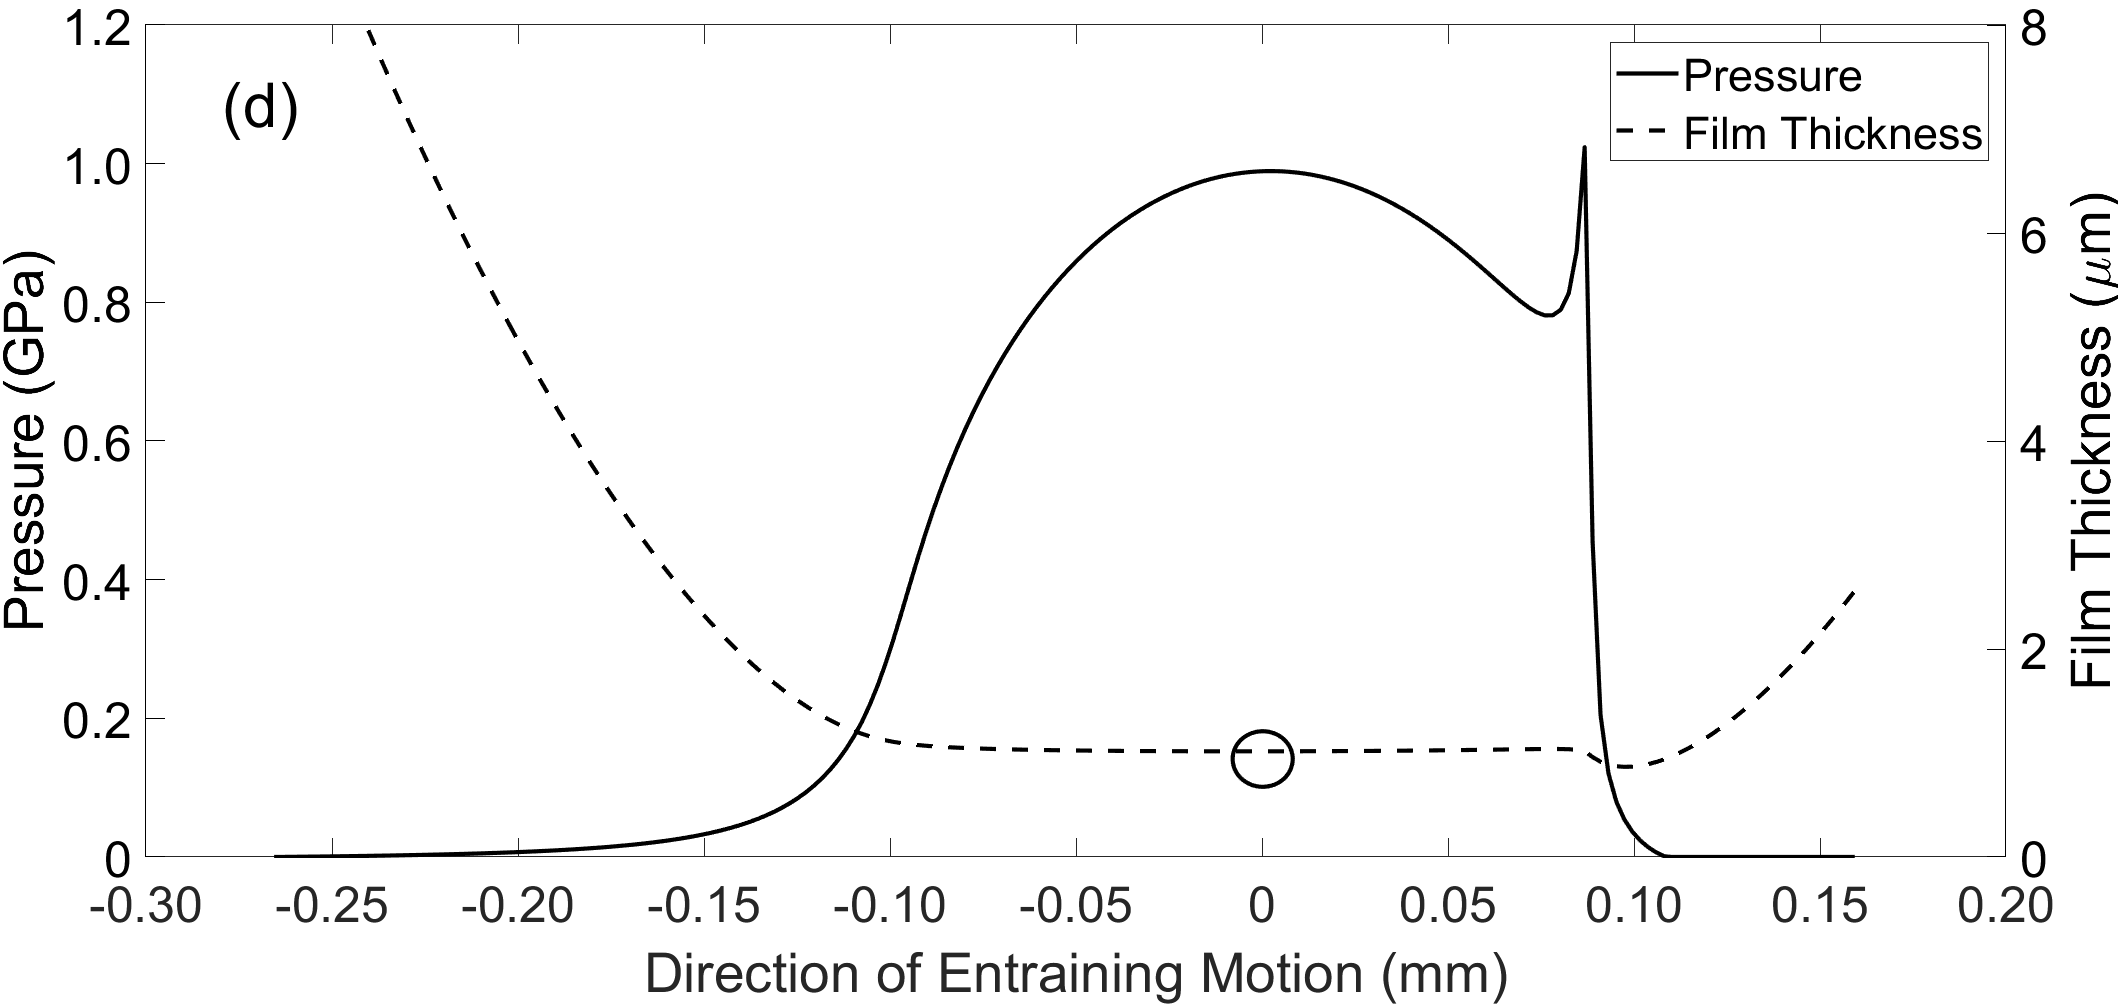
\includegraphics[width=\textwidth]{ExpTribo Figure 18d.png}
		\caption{}
		\label{NodeD}
	\end{subfigure}
	\hfill
	\begin{subfigure}[b]{0.49\textwidth}
		\centering
		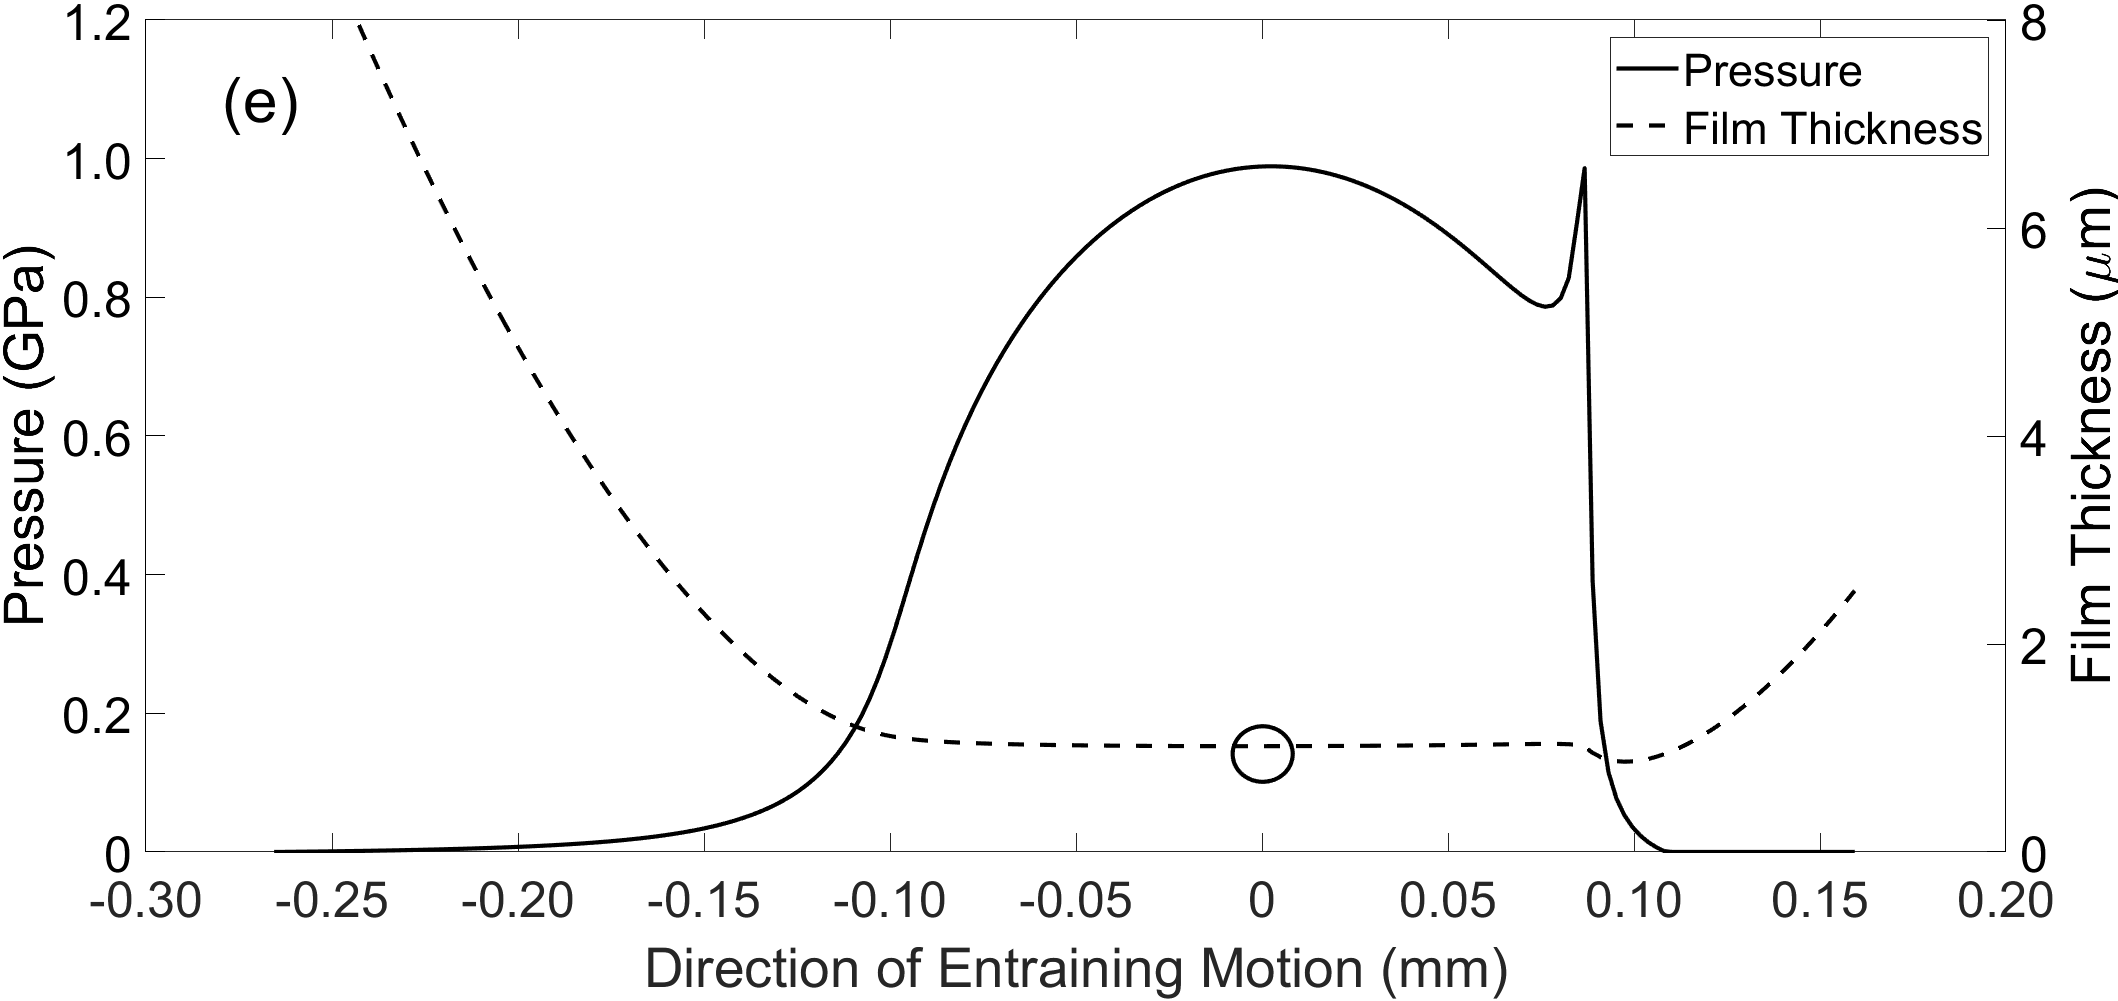
\includegraphics[width=\textwidth]{ExpTribo Figure 18e.png}
		\caption{}
		\label{NodeE}
	\end{subfigure}
	\hfill
	\begin{subfigure}[b]{0.49\textwidth}
		\centering
		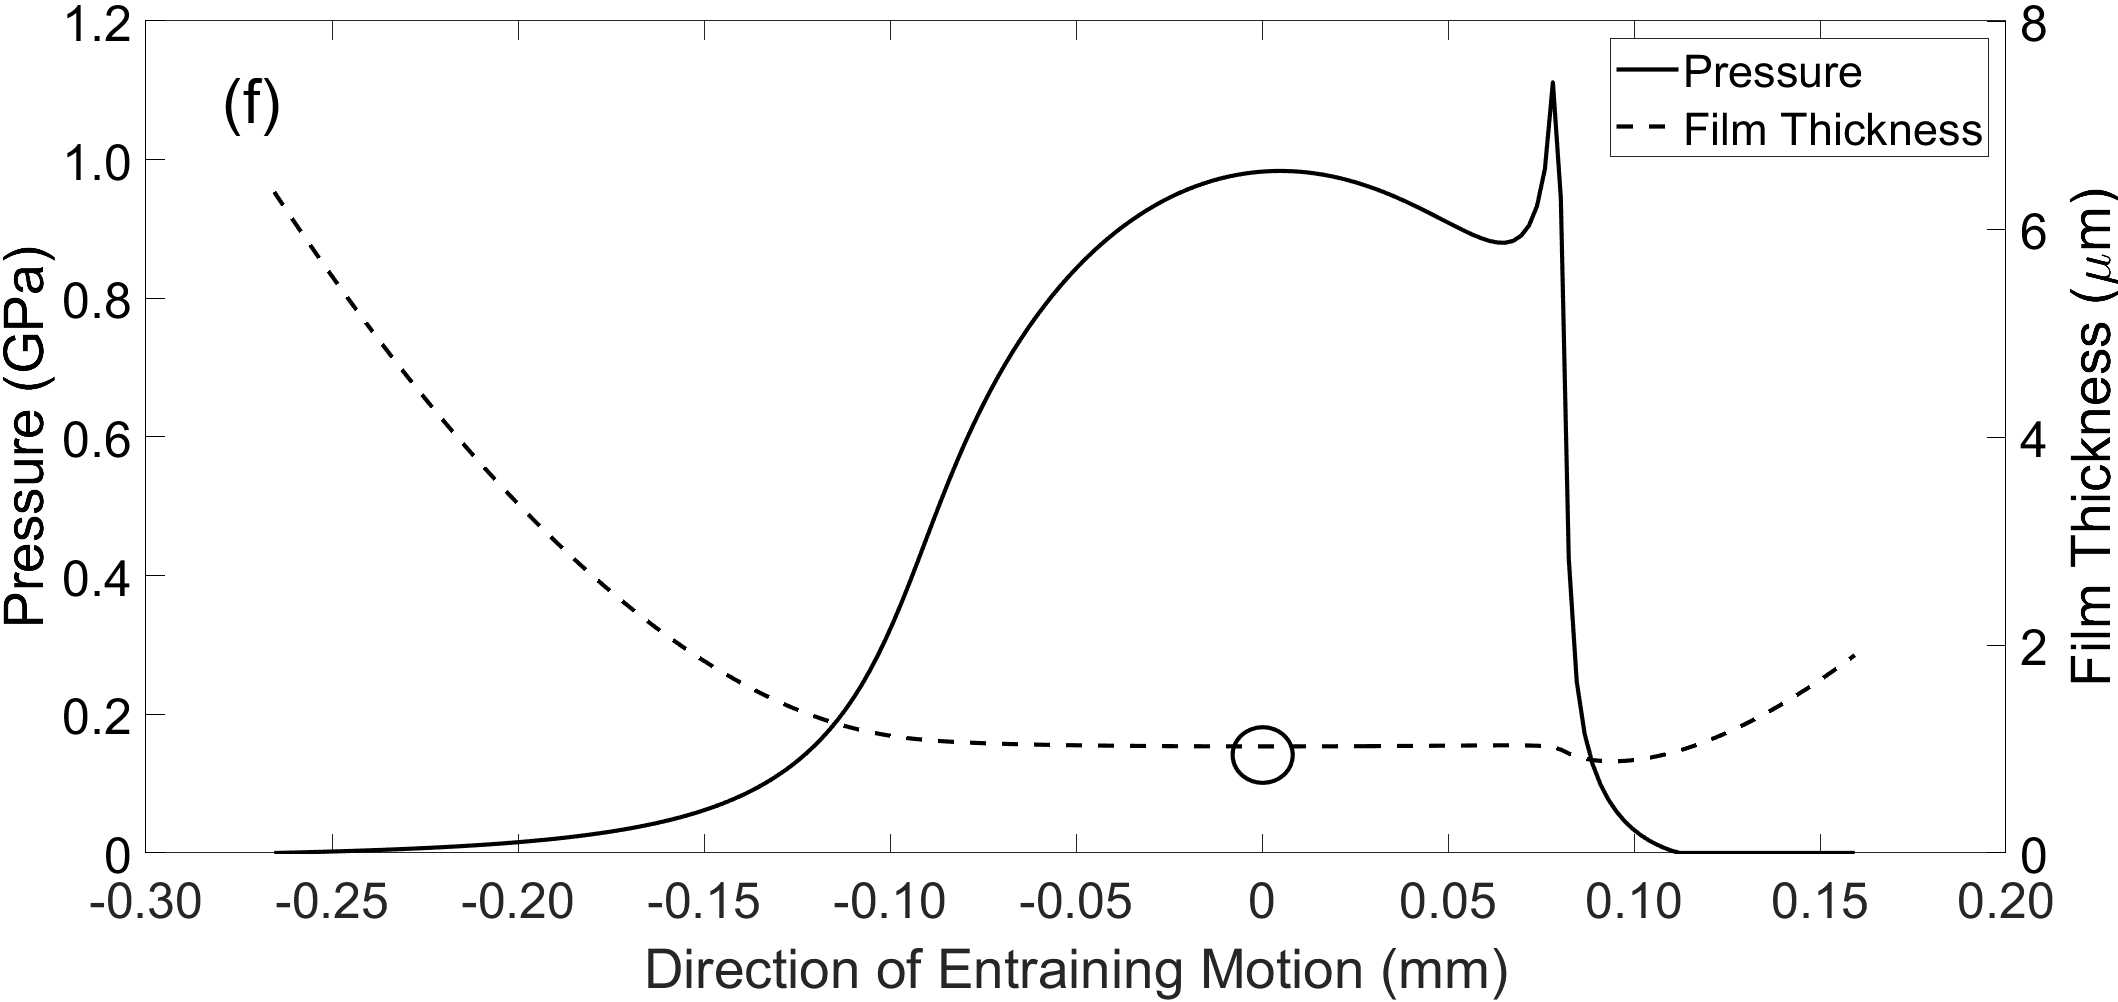
\includegraphics[width=\textwidth]{ExpTribo Figure 18f.png}
		\caption{}
		\label{NodeF}
	\end{subfigure}
	\caption{EHL pressure and film thickness distributions: a) Node 1, b) Node 2, c) Node 3, d) Node 4, e) Node 5, f) Node 6.}
	\label{EHL pressure and film thickness distributions}
\end{figure}

In each of these plots, it is possible again to see the central film thickness drop as the roller enters, then exits the loaded region. These central film values are represented by circles in Figure 18. Agreement between the extrapolated film formulae and the numerical model for calculating central film values are presented in Table \ref{Extrapolated film formulae and numerical model central film thickness comparison}. The extrapolated formula over-predicts the central film thickness by an average of 7.7\%, with a peak of 11.3\%. It is also shown that the central nodes which correspond to the higher loads in the loaded region have the lowest percentage difference in comparison to the lightly loaded nodes at the outer edges.

\begin{table*}
	%\captionsetup{justification=centering}
	\caption{Extrapolated film formulae and numerical model central film thickness comparison}
	\label{Extrapolated film formulae and numerical model central film thickness comparison}
	\centering
	\renewcommand{\arraystretch}{1.5}%
	\begin{tabular}{|P{0.08\textwidth}|P{0.35\textwidth}|P{0.35\textwidth}|P{0.18\textwidth}|}
		\hline
		\textbf{Node} & \textbf{Extrapolated Formulae Central Film Thickness ($\mu m$)} & \textbf{Numerical Model Central Film Thickness  ($\mu m$)} & \textbf{Percentage Difference (\%)} \\ [0.5ex]
		\hline
		1 & 1.142 & 1.026 & 11.3 \\ [0.5ex]
		\hline
		2 & 1.122 & 1.025 & 9.46 \\ [0.5ex]
		\hline
		3 & 1.075 & 1.019 & 5.49 \\ [0.5ex]
		\hline
		4 & 1.068 & 1.016 & 5.11 \\ [0.5ex]
		\hline
		5 & 1.072 & 1.018 & 5.30 \\ [0.5ex]
		\hline
		6 & 1.122 & 1.025 & 9.46 \\ [0.5ex]
		\hline
	\end{tabular}
\end{table*}

\section{Conclusions}

A novel methodology comprising experiments and numerical modelling was developed to allow component and conjunction level tribodynamic analysis of a roller bearing under speeds and loading conditions previously not reported. The experimental data contain the physics of the dynamics and tribology within the bearing, negating the need for a simplified and computationally intensive dynamic bearing model. The tribological conditions at the contact between an individual roller and raceways are numerically analysed. All lubrication regimes, including mixed-EHL and hydrodynamic, are considered as the roller passes through loaded and unloaded regions. The following conclusions can be made based on presented results:

\begin{enumerate}
	\item The contact experiences an order of magnitude increase in film thickness (0.1~-~1.9~$\mu m$) across the speed sweep from 0~-~15~000$rpm$. This leads to a 1~200~$N$ higher contact load for the analysis considering the EHL film implicitly when compared to the conventional dry modelling approach. This contact force difference is due to the EHL film acting as an interference element at the roller-race conjunction, leading to greater contact deformation.
	\item Further comparison between the dry and lubricated contact model reveals a percentage increase in load between both models of up to 149\% at 14~855~$rpm$. At lower speeds, and moderate loads, this increase is significantly lower, at just 14.8\%. During a period of system resonance at 14~135~$rpm$, where the dry contact deformation dominates over the film growth, this increase is only 25.1\% despite the high speed. These findings show that the most significant difference between modelling methods occurs at high entrainment velocities with low loads.
	\item The load values obtained from the lubricated tribological model have been used explicitly within a 1D EHL model to calculate the pressure distribution and film thickness across the contact. Employing the numerical EHL calculation explicitly negates the need for a computationally inefficient coupling of the numerical model at each sample point. At 8~350~$rpm$, the extrapolated formula over-predicts the central film thickness by an average of 7.7\%.
\end{enumerate}

This chapter introduced the importance of implicitly including the lubricant film in high-speed dynamic bearing models. At high speeds and low contact loads, the effect of the EHL film is shown to considerably affect the resulting contact forces. These operating conditions align with those of an input bearing in an electrified powertrain transmission, where input torque and hence bearing load decreases as rotational speeds increase. 

Additionally, this chapter introduced the fundamental tribological contact models and governing numerical methods used within this thesis. The contact methodology is further enhanced in the next chapter, and the 1D numerical model presented here will also be used for further analysis in the subsequent chapters. The next stage of these studies is to examine how this increase in contact load affects bearing and system dynamics under realistic electrified powertrain operating conditions. Due to the non-linear force-deflection relationship at the contact, the contact stiffness will also change. To answer the aims of this research, the effect of this stiffness must be analysed within a flexible system-level model,.